\chapter{Geometry}

\section{ Length of the union of line segments }
Given N line segments on the line, that is, each segment defined by a pair of coordinates ($X_1$, $X_2$). Consider the union of the segments and find its length.

The algorithm was proposed by Klee (Klee) in 1977. The algorithm works for the O (N log N). It was proved that this algorithm is faster (asymptotically).

\subsection{ Description }
We put all the coordinates of all segments in the array X and sort it by the value of the coordinates. An additional condition for sorting - with equal coordinates first must go left ends. In addition, for each element of the array will be stored, it is to the left or to the right end of the segment. Now go through the entire array, with counter C overlapping segments. If C is non-zero, then add the difference to the result of $X_i - X_{i-1}$. If the current element is to the left end, then increase the counter C, or else reduce it.

\subsection{ Implementation }
\begin{verbatim}
unsigned segments_union_measure (const vector <pair <int,int>> & a)
 {
     unsigned n = a.size();
     vector <pair <int,bool>> x (n * 2);
     for (unsigned i = 0; i <n; i++)
     {
         x [i * 2] = make_pair (a [i]. first, false);
         x [i * 2 +1] = make_pair (a [i]. second, true);
     }

     sort (x.begin(), x.end());

     unsigned result = 0;
     unsigned c = 0;
     for (unsigned i = 0; i <n * 2; i++)
     {
         if (c && i)
             result + = unsigned (x [i]. first - x [i-1]. first);
         if (x [i]. second)
            ++ C;
         else
             - C;
     }
     return result;
 } 
\end{verbatim}
\section{ Signed triangle area and "Clockwise" test }
\subsection{ Definition }

Given a three-point $p_1$, $p_2$, $p_3$. Find the value of \textbf{the sign area} $S$ Triangle $p_1 p_2 p_3$ i.e. area of ​​this triangle, taken with a plus or minus depending on the type of rotation formed by points $p_1$, $p_2$, $p_3$ : Anti-clockwise or her accordingly.

It is clear that if we learn how to calculate a symbolic ("targeted") area, and we can find the normal area of ​​any triangle, and will be able to check, clockwise or counter-directed any triple of points.

\subsection{ Calculation }

We use the notion \textbf{of a skew} (pseudoscalar) product of vectors. It just is twice the area of ​​the triangle sign:

$a \land b = | a | | b | \sin \angle (a, b) = 2 S,$

where the angle $\angle (a, b)$ taken oriented, i.e. is the angle of rotation between these vectors counterclockwise.

(Module twisted product of two vectors is equal to the modulus of \textbf{the vector} product.)

Bundle is calculated as the value of the determinant of the coordinates of the points:

$2S=\left|\begin{array}{ccc}
x_{1} & y_{1} & 1\\
x_{2} & y_{2} & 1\\
x_{3} & y_{3} & 1
\end{array}\right|$

Expanding the determinant, we can obtain the following formula:

$2S=x_{1}(y_{2}-y_{3})+x_{2}(y_{3}-y_{1})+x_{3}(y_{1}-y_{2})$

You can group the third term with the first two, getting rid of one multiplication:

$2S=(x_{2}-x_{1})(y_{3}-y_{1})-(y_{2}-y_{1})(x_{3}-x_{1})$

This formula is easy to record and store in a matrix form, as the following determinant:

$2S=\left|\begin{array}{cc}
x_{2}-x_{1} & y_{2}-y_{1}\\
x_{3}-x_{1} & y_{3}-y_{1}
\end{array}\right|$

\subsection{ Implementation }

Function that calculates the area of ​​a triangle twice landmark:

\begin{verbatim}
int triangle_area_2(int x1, int y1, int x2, int y2, int x3, int y3){
    return(x2 - x1)*(y3 - y1)-(y2 - y1)*(x3 - x1);
} 
\end{verbatim}
A function that returns the normal area of ​​a triangle:

\begin{verbatim}
double triangle_area(int x1, int y1, int x2, int y2, int x3, int y3){
    return abs(triangle_area_2(x1, y1, x2, y2, x3, y3)) / 2.0 ;
} 
\end{verbatim}
Function which checks whether the specified form triple points clockwise rotation:

\begin{verbatim}
bool clockwise(int x1, int y1, int x2, int y2, int x3, int y3){
    return triangle_area_2(x1, y1, x2, y2, x3, y3)< 0 ;
} 
\end{verbatim}
Function which checks whether the specified form triple points counterclockwise rotation:

\begin{verbatim}
bool counter_clockwise(int x1, int y1, int x2, int y2, int x3, int y3){
    return triangle_area_2(x1, y1, x2, y2, x3, y3)> 0 ;
} 
\end{verbatim}
\section{ Intersection of two segments }
Given two segments $AB$ and $CD$ (They can degenerate to a point). Want to check, cross or not.

If you want to find itself further point (s) of intersection, then refer to the corresponding article.

\subsection{ Using oriented area of ​​the triangle }

We use the oriented area of the triangle and a predicate 'Clockwise'. Indeed, the segments $AB$ and $CD$ intersect if and only if the point $A$ and $B$ on different sides of the line $CD$ And, similarly, the points $C$ and $D$ - On both sides of the line $AB$. You can check this by calculating the area of ​​the corresponding oriented triangles and comparing their signs.

The only thing you should pay attention to - the boundary cases where some points fall on the line itself. Thus there is only a special case where the above checks do not - the case where both segments \textbf{are} collinear. This case should be considered separately. It is sufficient to verify that the projections of these two segments on the axis $X$ and $Y$ intersect (often this test is called "test of the bounding box").

In general, this method - easier than the one that will be presented below (producing the intersection of two lines), and has fewer special cases, but its main drawback - the fact that he did not find the very intersection.

\textbf{Implementation:} \begin{verbatim}
struct pt {
    int x, y ;
} ;
 
inline int area(pt a, pt b, pt c){
    return(b. x - a. x)*(c. y - a. y)-(b. y - a. y)*(c. x - a. x);
}
 
inline bool intersect_1(int a, int b, int c, int d){
    if(a > b) swap(a, b);
    if(c > d) swap(c, d);
    return max(a,c)<= min(b,d);
}
 
bool intersect(pt a, pt b, pt c, pt d){
    return intersect_1(a. x, b. x, c. x, d. x )
        && intersect_1(a. y, b. y, c. y, d. y )
        && area(a,b,c)* area(a,b,d)<= 0
        && area(c,d,a)* area(c,d,b)<= 0 ;
} 
\end{verbatim}
In order to optimize the test for bounding box is moved to the beginning, to calculate the area - as it is more "easy" test.

Of course, this code applies to the case of real coordinates, just all comparisons with zero should be carried epsilon (and avoid the multiplication of two real-values $\rm area()$ By multiplying instead of signs).

\subsection{ Using the intersection of two lines }

Instead of crossing segments perform the intersection of two lines, as a result, if the lines are not parallel, we obtain some point you have to check it belongs to both segments, it is enough to check that this point belongs to both segments in the projection of the axis $X$ and axle $Y$.

If the line were parallel, then, if they do not match, the segments do not exactly overlap. If a direct match, the segments are on a line, and to check their intersection is sufficient to verify that the intersection of the projection of the axis $X$ and $Y$.

There is still a special case where one or both segments \textbf{degenerate} to the point: in this case, talking about direct incorrectly, and this method is not applicable (this case it will be necessary to disassemble separately).

\textbf{Sales} (excluding the case of degenerate intervals):

\begin{verbatim}
struct pt {
    int x, y ;
} ;
 
const double EPS = 1E-9 ;
 
inline int det(int a, int b, int c, int d){
    return a * d - b * c ;
}
 
inline bool between(int a, int b, double c){
    return min(a,b)<= c + EPS && c <= max(a,b)+ EPS ;
}
 
inline bool intersect_1(int a, int b, int c, int d){
    if(a > b) swap(a, b);
    if(c > d) swap(c, d);
    return max(a,c)<= min(b,d);
}
 
bool intersect(pt a, pt b, pt c, pt d){
    int A1 = a. y - b. y,  B1 = b. x - a. x,  C1 = - A1 * a. x - B1 * a. y ;
    int A2 = c. y - d. y,  B2 = d. x - c. x,  C2 = - A2 * c. x - B2 * c. y ;
    int zn = det(A1, B1, A2, B2);
    if(zn ! = 0){
        double x = - det(C1, B1, C2, B2)* 1. / zn ;
        double y = - det(A1, C1, A2, C2)* 1. / zn ;
        return between(a. x, b. x, x)&& between(a. y, b. y, y )
            && between(c. x, d. x, x)&& between(c. y, d. y, y);
    }
    else
        return det(A1, C1, A2, C2)== 0 && det(B1, C1, B2, C2)== 0
            && intersect_1(a. x, b. x, c. x, d. x )
            && intersect_1(a. y, b. y, c. y, d. y);
} 
\end{verbatim}
It first calculates the $\rm zn$ - The denominator in Kramer. If ${\rm zn} = 0$, The coefficients $A$ and $B$ direct proportional, and the lines are parallel or coincide. In this case, you should check whether or not they are the same, which is necessary to check that the coefficients $C$ is directly proportional to the same factor, which is sufficient to compute the determinant of the following two if they are both equal to zero, then the lines are the same:

$\left|\begin{array}{cc}
A_{1} & C_{1}\\
A_{2} & C_{2}
\end{array}\right|,\left|\begin{array}{cc}
B_{1} & C_{1}\\
B_{2} & C_{2}
\end{array}\right|$

If the ${\rm zn} \ne 0$, The lines intersect, and Cramer's rule we find the point of intersection $(X, y)$ and verify that it belongs to both segments.

It should be noted that if the initial coordinates of the points have already been real-valued, we must normalize the direct (i.e., to bring them to such a state that the sum of squares of the $a$ and $b$ equal to one), otherwise error when compared to the parallel lines and a match may be too large.

\section{ Equation of the line for the segment }
Task - given the coordinates of the end of the segment to build a line through it.

We believe that the segment is non-degenerate, i.e., has a length greater than zero (otherwise, of course, passes through an infinite number of different lines).

\subsection{ Two-dimensional case }

Given a segment $PQ$ i.e. the coordinates of its end $P_x$, $P_y$, $Q_x$, $Q_y$.

Required to construct a \textbf{linear equation for the plane} through this segment, i.e. find the coefficients $A$, $B$, $C$ in the equation of the line:

$A x + B y + C = 0.$

Note that the required triples $(A, B, C)$ Passing through a given segment, \textbf{there are infinitely many:} you can multiply the three terms on any non-zero number and get the same line. Therefore, our task - to find one of these triples.

It is easy to see (by substituting these expressions and the coordinates of points $P$ and $Q$ in the equation of the line), which fits the following set of factors:

$A = P_y - Q_y,$
$B = Q_x - P_x,$
$C = - A P_x - B P_y.$

\subsubsection{ Integer case }

An important advantage of this method of construction of the line is that if all the coordinates are integers, then the obtained coefficients are also \textbf{integers.} In some cases, this allows geometric operations, generally without the real numbers.

However, there is a small drawback: one and the same line can be prepared three different ratios. To avoid this, but do not go from integer coefficients, you can use this technique, often called \textbf{a valuation.} We find the greatest common divisor of the numbers $| A |$, $| B |$, $| C |$, Divide it by three terms, and then we make the sign of the normalization: if $A <0$ or $A = 0, B <0$ Then multiply the three terms on the $-1$. In the end, we will come to that same direct shall receive the same three factors that make it easy to check the lines on equality.

\subsubsection{ The real-valued case }

When working with real numbers must always remember the errors.

The coefficients $A$ and $B$ we obtained about the original coordinates, the coefficient $C$ - Is the order of the square of them. It may already be large enough numbers, and, for example, the intersection of lines, they will be even more, which can lead to large rounding errors, even at the original coordinates of the order $10 ^ 3$.

Therefore, when working with real numbers is desirable to produce the so-called \textbf{normalization of the} line: namely, to make the coefficients such that $A ^ 2 + B ^ 2 = 1$. To do this, we need to calculate the number of $Z$ :

$Z = \sqrt {A ^ 2 + B ^ 2}$

and share all three coefficients $A$, $B$, $C$ at him.

Thus, the order of the coefficients $A$ and $B$ will not depend on the order of the input coordinates, and the coefficient $C$ is of the same order as the input coordinates. In practice, this leads to a significant improvement in precision.

Finally, we mention the direct \textbf{comparison} - because after such a normalization for one and the same line may be produced only two triples format: up to multiplication by $-1$. Accordingly, if we make additional normalization with sign (if $A <- \varepsilon$ or $| A | <\varepsilon, B <- \varepsilon$ Then multiply by $-1$ ), The resulting coefficients are unique.

\subsection{ Three-dimensional and multi-dimensional case }

Already in three dimensions \textbf{there is no simple equation that} describes the line (it can be defined as the intersection of two planes, i.e., a system of two equations, but it is inconvenient way).

Consequently, the three-dimensional and multi-dimensional cases, we have to use \textbf{a parametric method of defining line,} i.e. as a point $p$ and a vector $v$ :

$p + v t, ~ ~ ~ t \in \cal {R}.$

i.e. straight - all points that can be obtained from the point $p$ adding vector $v$ with an arbitrary coefficient.

\textbf{Construction of} the line in parametric form by end point of the segment - is trivial, we just take one end of the segment as a point $p$, And the vector from the first to the second end - for the vector $v$.

\section{ Intersection point }
Suppose we are given two lines defined by their coefficients $A_1, B_1, C_1$ and $A_2, B_2, C_2$. Need to find their point of intersection, or to find out what the lines are parallel.

\subsection{ Decision }

If two lines are not parallel, then they intersect. To find a point of intersection of the two is enough to make a direct system of equations and solve it:

$\begin{cases}
A_{1}x+B_{1}y+C_{1}=0\\
A_{2}x+B_{2}y+C_{2}=0
\end{cases}$

Using Cramer's rule, we find the right solution, which is the desired \textbf{point of intersection:}

$$ x=-\frac{\left|\begin{array}{cc}
C_{1} & B_{1}\\
C_{2} & B_{2}
\end{array}\right|}{\left|\begin{array}{cc}
A_{1} & B_{1}\\
A_{2} & B_{2}
\end{array}\right|}=-\frac{C_{1}B_{2}-C_{2}B_{1}}{A_{1}B_{2}-A_{2}B_{1}}$$

$$ y=-\frac{\left|\begin{array}{cc}
A_{1} & C_{1}\\
A_{2} & C_{2}
\end{array}\right|}{\left|\begin{array}{cc}
A_{1} & B_{1}\\
A_{2} & B_{2}
\end{array}\right|}=-\frac{A_{1}C_{2}-A_{2}C_{1}}{A_{1}B_{2}-A_{2}B_{1}}$$

If the denominator is zero, that

$ $$\left|\begin{array}{cc}
A_{1} & B_{1}\\
A_{2} & B_{2}
\end{array}\right|=A_{1}B_{2}-A_{2}B_{1}=0$

then the system has no solutions (the lines are \textbf{parallel} and do not coincide) or infinitely many (straight \textbf{match).} If it is necessary to distinguish between these two cases, it is necessary to check that the coefficients $C$ is directly proportional to the same aspect ratio as the coefficients $A$ and $B$, Which is enough to calculate the determinant of the two if they are both equal to zero, then the lines are the same:
$\left|\begin{array}{cc}
A_{1} & C_{1}\\
A_{2} & C_{2}
\end{array}\right|,\left|\begin{array}{cc}
B_{1} & C_{1}\\
B_{2} & C_{2}
\end{array}\right|$

\subsection{ Implementation }

\begin{verbatim}
struct pt {
    double x, y ;
} ;
 
struct line {
    double a, b, c ;
} ;
 
const double EPS = 1e-9 ;
 
double det(double a, double b, double c, double d){
    return a * d - b * c ;
}
 
bool intersect(line m, line n, pt & res){
    double zn = det(m. a, m. b, n. a, n. b);
    if(abs(zn)< EPS )
        return false ;
    res. x = - det(m. c, m. b, n. c, n. b)/ zn ;
    res. y = - det(m. a, m. c, n. a, n. c)/ zn ;
    return true ;
}
 
bool parallel(line m, line n){
    return abs(det(m. a, m. b, n. a, n. b)) < EPS ;
}
 
bool equivalent(line m, line n){
    return abs(det(m. a, m. b, n. a, n. b)) < EPS
        && abs(det(m. a, m. c, n. a, n. c)) < EPS
        && abs(det(m. b, m. c, n. b, n. c)) < EPS ;
} 
\end{verbatim}
\section{ Intersection of the two segments }
Given two segments $AB$ and $CD$ (They can degenerate to a point). Need to find their intersection: it may be empty (if the segments do not overlap), can be a single point, and can be a whole segment (if the segments are superimposed on each other).

\subsection{ Algorithm }

Segments will work with both direct us build on the two segments of direct equation, checking whether parallel lines. If the lines are not parallel, it's simple: we find their point of intersection, and verify that it belongs to both segments (it is enough to verify that the point belongs to each segment in the projection on the axis $X$ and axle $Y$ separately). As a result, in this case, the answer is either "empty" or only this location.

A more complex case - if the lines were parallel (same applies here a case where one or both segments degenerated into points). In this case it is necessary to check that both segments are collinear (or, in the case when both are degenerate to the point - that this point is the same). If it is not, then the answer is - "empty." If so, then the answer is - it's the intersection of two segments lying on the same line, that's simple enough - we have to take up all of the left and right ends of the minimum.

At the beginning of the algorithm will write so-called "check for bounding box" - first, it is necessary for the case where two segments are collinear, and secondly, it is a lightweight verification, allows the algorithm to work faster on the average random tests.

\subsection{ Implementation }

We present here the full implementation, including all support functions for working with points and lines.

The main feature here is the $\rm intersect$, Which intersects two segments assigned to it, and if they meet at least one point, then returns $\rm true$ And the arguments $\rm left$ and $\rm right$ returns the start and end of the segment, the response (in particular, when the answer - it is the only point that is returned will be the beginning and end of the match).

\begin{verbatim}
const double EPS = 1E-9 ;
 
struct pt {
    double x, y ;
 
    bool operator <(const pt & p)const {
        return x < p. x - EPS || abs(x - p. x)< EPS && y < p. y - EPS ;
    }
} ;
 
struct line {
    double a, b, c ;
 
    line() { }
    line(pt p, pt q){
        a = p. y - q. y ;
        b = q. x - p. x ;
        c = - a * p. x - b * p. y ;
        norm() ;
    }
 
    void norm() {
        double z = sqrt(a * a + b * b);
        if(abs(z)> EPS )
            a / = z,  b / = z,  c / = z ;
    }
 
    double dist(pt p)const {
        return a * p. x + b * p. y + c ;
    }
} ;
 
#define det(a,b,c,d)  (a*d-b*c)
 
inline bool betw(double l, double r, double x){
    return min(l,r)<= x + EPS && x <= max(l,r)+ EPS ;
}
 
inline bool intersect_1d(double a, double b, double c, double d){
    if(a > b) swap(a, b);
    if(c > d) swap(c, d);
    return max(a, c)<= min(b, d)+ EPS ;
}
 
bool intersect(pt a, pt b, pt c, pt d, pt & left, pt & right){
    if(! intersect_1d(a. x, b. x, c. x, d. x)|| ! intersect_1d(a. y, b. y, c. y, d. y))
        return false ;
    line m(a, b);
    line n(c, d);
    double zn = det(m. a, m. b, n. a, n. b);
    if(abs(zn)< EPS){
        if(abs(m. dist(c)) > EPS || abs(n. dist(a)) > EPS )
            return false ;
        if(b < a) swap(a, b);
        if(d < c) swap(c, d);
        left = max(a, c);
        right = min(b, d);
        return true ;
    }
    else {
        left. x = right. x = - det(m. c, m. b, n. c, n. b)/ zn ;
        left. y = right. y = - det(m. a, m. c, n. a, n. c)/ zn ;
        return betw(a. x, b. x, left. x )
            && betw(a. y, b. y, left. y )
            && betw(c. x, d. x, left. x )
            && betw(c. y, d. y, left. y);
    }
} 
\end{verbatim}
\section{ Area of a simple polygon }
Given a simple polygon (i.e. without self-intersections, but not necessarily convex), given the coordinates of its vertices in order to circumvent or counter-clockwise. Want to find its area.

\subsection{ Method 1 }
This is easy to do if through all the edges and fold the area of ​​a trapezoid bounded by each edge. The area must be taken with the sign with which it happens (thanks to mark all the "extra" area will be reduced.) i.e. formula is:

\begin{verbatim}
S + = (X2 - X1) * (Y1 + Y2) / 2 
\end{verbatim}
Code:

\begin{verbatim}
double sq (const vector <point> & fig)
 {
     double res = 0;
     for (unsigned i = 0; i <fig.size(); i++)
     {
         point
             p1 = i?  fig [i-1]: fig.back(),
             p2 = fig [i];
         res + = (p1.x - p2.x) * (p1.y + p2.y);
     }
     return fabs (res) / 2;
 } 
\end{verbatim}\subsection{ Method 2 }
Can proceed in another way. Choose an arbitrary point O, iterate through all edges, adding to the response-oriented area of the triangle formed by the edge and the point O (see oriented area of the triangle ). Again, thanks to the sign, the entire extra space will be reduced, and will only answer.

This method is good because it's easier to be extended to more complex cases (for example, when some parties - not direct, but the arc of the circle).

\section{ Area of ​​a lattice polygon (Pick's Theorem) }
Polygon without self-called lattice if all its vertices are at the points with integer coordinates (in Cartesian coordinates).

\subsection{ Pick's Theorem }

\subsubsection{ Formula }

Let there be given a trellis polygon with non-zero area.

Denote its area by $S$, The number of points with integer coordinates lying strictly inside the polygon - through $I$, The number of points with integer coordinates that lie on the sides of the polygon - through $B$.

Then, the relation, called \textbf{Pick's formula:}

$S = I + \frac {B} {2} - 1.$

In particular, if the values ​​of I and B for some of the polygon, the surface area can be calculated for $O (1)$ Without knowing the coordinates of its vertices.

This relation is discovered and proved the Austrian mathematician Georg Alexander Pick (Georg Alexander Pick) in 1899

\subsubsection{ Proof }

The proof is in several steps from simple shapes to arbitrary polygons:

The unit square. In fact, for him $S = 1$, $I = 0$, $B = 4$, And the formula is correct.
Arbitrary non-degenerate rectangle with sides parallel to the axes. To prove denote $a$ and $b$ the length of the rectangle. Then we find: $S = ab$, $I = (a-1) (b-1)$, $B = 2 (a + b)$. Direct substitution, we see that the formula is correct Peak.
Right triangle with legs parallel to the coordinate axes. For proof, we note that any such triangle can be obtained by cutting off some of its diagonal rectangle. Denoting $c$ the number of integral points on the diagonal, it can be shown that the formula holds for Pick such a triangle, regardless of the $c$.
Arbitrary triangle. Note that any such triangle can be turned into a rectangle sticking to the sides of right triangles with legs parallel to the axes (in this case need no more than three of these triangles). From here you can get the correct formula for Pick any triangle.
Arbitrary polygon. To prove triangulate it, i.e. divided into triangles with vertices at integer points. For a triangle formula Peak we have already proved. Further, it can be shown that the addition of an arbitrary polygon Pick any triangle formula retains its validity. By induction, it follows that it is true for any polygon.
\subsection{ Generalization to higher dimensions }

Unfortunately, this is so simple and beautiful formula Pick bad generalized to higher dimensions.

Demonstrated this Reeve (Reeve), proposing in 1957 to consider the tetrahedron (now called \textbf{Riva tetrahedron)} with the following peaks:

$A = (0,0,0),$
$B = (1,0,0),$
$C = (0,1,0),$
$D = (1,1,k)$

where $k$ - Any positive integer. Then this tetrahedron $ABCD$ at any $k$ does not contain the single point with integer coordinates, and on its border - lie just four points $A$, $B$, $C$, $D$ and no other. Thus, the volume and surface area of ​​the tetrahedron can be different, while the number of points inside and on the border - are unchanged, therefore, the formula does not allow for generalizations Pick even three-dimensional case.

However, such a generalization to higher dimensions is still there - it \textbf{Ehrhart polynomials} (Ehrhart Polynomial), but they are quite complex and depend not only on the number of points inside and on the border of the shape.

\section{ Point cover for a set of segments }
Given N line segments on the line. Required to cover their fewest points, i.e. find the smallest set of points such that each segment belongs to at least one point.

We also consider the more complicated version of this problem - when Adding a "prohibited" a set of segments, i.e. no point of the answer should not belong to any prohibited segment.

It should also be noted that this problem can be viewed as a problem in scheduling theory - it is required to cover a given set of events-segments fewest points.

Below we describe a greedy algorithm that solves both problems for the \textbf{O (N log N).}

\subsection{ The first task }
Note first that we can consider only those solutions in which each point is located at the right end of a segment. Indeed, it is easy to see that any solution, if it does not satisfy this property, we can bring to it, shifting it to the right point to the extent possible.

Let us now try to build a solution that meets the specified property. Choose points-right ends of the segments, sort them, and move on them from left to right. If the current point is the right end of the segment is already covered, we skip it. Suppose now that the current point is the right end of this segment, which has not been covered before. Then we have to add in response to the current location, and mark all the pieces that hold this point of the coating. Indeed, if we missed the current point and would not add it to the answer, because it is the right end of this interval, then we will not be able to cover the current segment.

However, the naive implementation of this method will work for the O (N 2). We describe \textbf{an efficient implementation} of this method.

Take all the points are the ends of segments (both left and right) and sort them. In this case, for each save with her room segment, and also how it is the end of it (left or right). In addition, the sort point so that if there are a few points with one coordinate, it will first go to the left end, and only then - right. Head of the stack, which will be stored number of segments covered in this time; originally stack is empty. We move on to the points in sorted order. If the current point - the left end, then just add the number of its segment in the stack. If it is the right end, then check that it has not covered this segment (you can just make a list of boolean variables). If he has already been covered, then do nothing and go to the next point (looking ahead, we argue that in this case, the stack of the current segment is not.) If it has not been covered, we add the current point in the answer, and now we want to note for all current lines, they are covered. Since the stack is just numbers stored uncovered more segments, then we will get one from the stack segment, and notes that it is already covered, until the stack is completely empty. At the end of the algorithm all the segments will be covered, and, moreover, the least number of points (again, it is important to request that the case of equality of origin first go left end, and only then to the right.)

Thus, the entire algorithm runs in O (N), not counting the sort of points, and the resulting complexity of the algorithm is exactly equal to \textbf{O (N log N).}

\subsection{ The second task }
Here are emerging prohibited segments, so, first, the solution may not exist at all, and secondly, we can not say that the answer can be only of the right ends of the segments. However, the above algorithm can be suitably modified.

Again, we take all the point-ends of the segments (as target segments, and the forbidden), sort them and preserve each of its type and length, the end of which she is. Again, sort the pieces so that coordinates with equal left endpoints were to the right, and if all types are equal, the left ends of the prohibition must go to the left end of the target, and the right ends of the banned - after the target (to illegal segments into account as long as possible with equal coordinates). Head count of prohibited segments, which will be equal to the number of prohibited intervals, covering the current point. Head of the queue (queue), in which to store the current number of target segments. We will sort out the points in sorted order. If the current point - the left end of the target segment, just add the number of the segment in its place. If the current point - right end of the target segment, if the counter is prohibited segments is zero, then we do the same previous problem - put an end to the current location, and pushes all the segments of the line, noting that they are covered. If the counter is prohibited intervals greater than zero, the current point, we can not shoot, so we have to find the last point that is free from prohibited segments, and for this it is necessary to maintain an appropriate pointer last\_free, which will be updated when you receive a forbidden segments. Then we shoot in last\_free-EPS (because it just can not be shot - this point is a disallowed segment), and push the pieces out of the queue until the point last\_free-EPS belongs to them. Namely, if the current point - the left end of the forbidden interval, then we increment the counter, and if before the counter is equal to zero, then assign last\_free current position. If the current point - right end of the forbidden interval, simply decrease the counter.

\section{ Centroids of polygons and polyhedra }
\textbf{The center of gravity} (or \textbf{center of mass)} of a body is the point with the property that if a body hanging over this point, it will maintain its position.

The following are the two-dimensional and three-dimensional problems associated with finding different mass centers - mostly in terms of computational geometry.

In the solutions discussed below are two basic \textbf{facts.} The first - that the center of mass of the material points equal to the average of their coordinates, taken with coefficients proportional to their masses. The second finding - that if we know the mass centers of two disjoint pieces, the center of mass of their union will be on the segment connecting the two centers, and it will divide it in the same proportion as the mass of the second figure refers to the weight of the first.

\subsection{ Two-dimensional case: polygons }

In fact, speaking of the center of mass of the two-dimensional shapes, you keep in mind one of the following three \textbf{objectives:}

The center of mass of the system of points - i.e. all mass is concentrated only at the vertices of the polygon.
The center of mass frame - that is, weight polygon focused on its perimeter.
Center of mass of the solid figures - i.e. weight polygon distributed throughout its area.
Each of these tasks is an independent decision, and will be discussed separately below.

\subsubsection{ Center of mass of a system of points }

This is the easiest of the three tasks, and its solution - known physical formula the center of mass system of particles:

$\vec{r_{c}}=\frac{\sum_{i}\vec{r_{i}}m_{i}}{\sum_{i}m_{i}}$

where $m_i$ - The mass points $\vec {r_i}$ - Their position vectors (defining their position relative to the origin), and $\vec {r_c}$ - The search radius vector of the center of mass.

In particular, if all the points have the same mass, the coordinates of the center of mass is the \textbf{arithmetic mean} of point coordinates. For a \textbf{triangle,} this point is called the \textbf{centroid} coincides with the intersection of media:

$\vec{r_{c}}=\frac{\vec{r_{1}}+\vec{r_{2}}+\vec{r_{3}}}{3}$

To \textbf{prove} these formulas is enough to recall that the equilibrium is reached at a point $r_c$ In which the sum of all forces is zero. In this case, it becomes the condition that the sum of the radius vectors of the points relative to the point $r_c$, Multiplied by the mass of the corresponding points, equal to zero:

$\sum_{i}(\vec{r_{i}}-\vec{r_{c}})m_{i}=\vec{0}$

and expressing here $\vec {r_c}$, We obtain the required formula.

\subsubsection{ Center of mass of a frame }

We assume for simplicity that the frame is uniform, i.e. its density is everywhere the same.

But then each side of the polygon can be replaced by a single point - the middle of this segment (as the center of mass of a homogeneous segment is the middle of this segment), with a mass equal to the length of this segment.

Now we have the problem of a system of material points, and apply the solution of the previous section, we find:

$\vec{r_{c}}=\frac{\sum_{i}\vec{r'_{i}}l_{i}}{P}$

where $\vec {r_i ^ \prime}$ - Point-to-mid $i$ The second side of the polygon, $l_i$ - Length $i$ The second part, $P$ - The perimeter, i.e. the sum of the lengths of sides.

For a \textbf{triangle} can show the following statement: This point \textbf{is} the \textbf{intersection of the bisectors} of the triangle formed by the midpoints of the sides of the original triangle. (To show this, we use the above formula, and then notice that the bisector divided by a triangle in the same ratio as the centers of mass of the parties).

\subsubsection{ Center of mass of a solid figure }

We believe that mass is distributed uniformly on the figure, that is, density at each point of the figure is equal to the same number.

The case of the triangle
States that for a triangle answer is still the same \textbf{centroid,} i.e. point formed by the arithmetic mean of the coordinates of the vertices:

$\vec{r_{c}}=\frac{\vec{r_{1}}+\vec{r_{2}}+\vec{r_{3}}}{3}$

The case of a triangle: proof
We give here an elementary proof that does not use the theory of integrals.

Like the first, purely geometric proof led Archimedes, but it was very complicated, with a large number of geometric constructions. The proof given here is taken from an article Apostol, Mnatsakanian "Finding Centroids the Easy Way".

The proof comes down to, to show that the center of mass of the triangle lies on one of the medians, and repeat this process two more times, we thus show that the center of mass lies at the intersection of the median, which is the centroid.

We divide this triangle $T$ four by connecting the midpoints of sides, as shown in the figure:

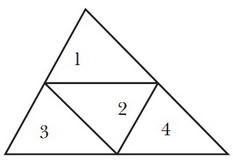
\includegraphics[scale=0.5]{1.jpg}

Four a triangle similar triangle $T$ a factor $1/2$.

Triangles number 1 and number 2 together form a parallelogram, whose center of mass $c_ {12}$ lies at the intersection of its diagonals (as this figure is symmetric with respect to both diagonals, and, hence, its center of mass must lie on each of the two diagonals). Point $c_ {12}$ in the middle part of the overall triangle number 1 and number 2, and lies on the median of a triangle $T$ :

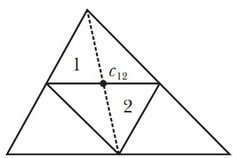
\includegraphics[scale=0.5]{2.jpg}

Now let the vector $\vec {r}$ - Vector from the top $A$ the center of mass $c_1$ Triangle number 1, and that the vector $\vec {m}$ - Vector from $A$ to the point $c_ {12}$ (Which, we recall, is the midpoint of the side on which it is):

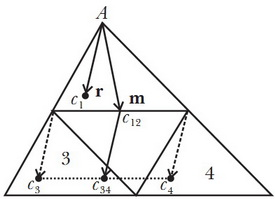
\includegraphics[scale=0.5]{3.jpg}

Our goal - to show that the vector $\vec {r}$ and $\vec {m}$ collinear.

We denote $c_3$ and $c_4$ points that are the centers of mass of the triangles number 3 and number 4. Then, obviously, the center of mass of the combination of these two triangles will be the point $c_ {34}$, Which is the midpoint of $c_3 c_4$. Furthermore, the vector from point $c_ {12}$ to the point $c_ {34}$ coincides with the vector $\vec {r}$.

Seeking the center of mass $c$ Triangle $T$ lies in the middle of the segment connecting the points $c_ {12}$ and $c_ {34}$ (Because we have broken the triangle $T$ into two equal areas: nº 1 - nº 2 and nº 3 - nº 4):

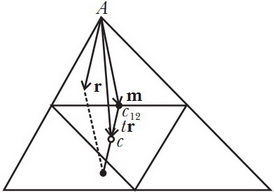
\includegraphics[scale=0.5]{4.jpg}

Thus, the vector from the vertex $A$ to the centroid $c$ is $\vec {m} + \vec {r} / 2$. On the other hand, since nº 1 triangle similar to the triangle $T$ a factor $1/2$, The same vector is $2 \vec {r}$. Hence we obtain the equation:

$\vec {m} + \vec {r} / 2 = 2 \vec {r},$

from which we find:

$\vec {r} = \frac {2} {3} \vec {m}.$

Thus, we have proved that the vector $\vec {r}$ and $\vec {m}$ collinear, which means that it has the centroid $c$ lies on the median, coming from the top $A$.

Moreover, along the way we have proved that the centroid divides each median for $2:1$ Starting from the top.

The case of a polygon
We now turn to the general case - that is, \textbf{mnougougolnika} the case. For him, such arguments are no longer applicable, so we reduce the problem to a triangle: namely, that we split the polygon into triangles (i.e. triangulate it), we find the center of mass of each triangle, and then find the center of mass of the mass centers of the resulting triangles.

The final formula is obtained as follows:

$\vec{r_{c}}=\frac{\sum_{i}\vec{r_{i}^{\text{o}}}S_{i}}{S}$

where $\vec {r_i ^ \circ}$ - Centroid $i$ The first triangle in the polygon triangulation, $S_i$ - Area $i$ On the triangle of the triangulation $S$ - The area of ​​a polygon.

Triangulation of a convex polygon - a trivial task for this, for example, can take the triangles $(R_1, r_ {i-1}, r_i)$ Where $i = 3 \ldots n$.

The case of a polygon: an alternative way
On the other hand, the application of this formula is not very convenient \textbf{for} non-convex \textbf{polygons,} since they produce a triangulation - in itself a difficult task. But for these polygons can think of a simpler approach. Specifically, the analogy with the way you can search the area of ​​an arbitrary polygon: Select an arbitrary point $z$ And then added the sign area of ​​the triangle formed by that point and the points of the polygon: $S = | \sum_ {i = 1} ^ n S_ {z, p_i, p_ {i +1}} |$. A similar technique can be applied to find the center of mass: only now we will summarize the centers of mass of the triangles $(Z, p_i, p_ {i +1})$ Taken with a coefficient proportional to their areas, i.e. The final formula for the center of mass is:

$$\vec{r_{c}}=\frac{\sum\vec{r_{z,p_{i},p_{i+1}}^{\text{o}}}S_{z,p_{i},p_{i+1}}}{S}$$

where $z$ - An arbitrary point, $p_i$ - Points of a polygon, ${\Vec r} _ {z, p_i, p_ {i +1}} ^ \circ$ - The centroid of the triangle $(Z, p_i, p_ {i +1})$, $S_ {z, p_i, p_ {i +1}}$ - The sign area of ​​the triangle, $S$ - The sign area of ​​a polygon (i.e. $S = \sum_ {i = 1} ^ {n} S_ {z, p_i, p_ {i +1}}$ ).

\subsection{ Three dimensions: the polyhedra }

Similarly, two-dimensional case, in 3D, you can talk directly to the four possible formulations of the problem:

The center of mass of the system of points - the vertices of.
The center of mass frame - edges of a polyhedron.
Center of mass of the surface - that is, mass is distributed over the surface area of ​​the polyhedron.
The center of mass of solid polyhedron - i.e. mass is distributed throughout the polyhedron.
\subsubsection{ Center of mass of the system of points }

As in the two-dimensional case, we can use physical formula and get the same result:

$\vec{r_{c}}=\frac{\sum_{i}\vec{r_{i}}m_{i}}{\sum_{i}m_{i}}$

which in the case of equal masses becomes average coordinates of all points.

\subsubsection{ Center of mass of the frame of the polyhedron }

Similarly, two-dimensional case, we simply replace each edge of the polyhedron material point, around the middle of the edge, and with a mass equal to the length of the edge. To get the problem of material points, we can easily find the solution as a weighted sum of the coordinates of these points.

\subsubsection{ Center of mass of the surface of the polyhedron }

Each face of the polyhedron surface - two-dimensional figure, the center of mass which we know how to look. Finding these centers of mass and replacing every facet of its center of mass, we obtain a problem with the material points, which is easy to solve.

\subsubsection{ Center of mass of solid polyhedron }

The case of a tetrahedron
As in the two-dimensional case, we solve first the simplest task - a task for the tetrahedron.

States that the center of mass of the tetrahedron is the point of intersection of its medians (median tetrahedron is called a segment drawn from the vertices to the center of mass of the opposite face, so the median tetrahedron passes through the top and through the intersection of the median triangular faces).

Why is this so? Here are correct arguments similar two-dimensional case, if we cut the tetrahedron on two tetrahedra with a plane passing through the top of the tetrahedron and some median opposite face, then both get a tetrahedron will be the same (as the triangular face is broken into two median triangles of equal area, and the height of two tetrahedrons not change). Repeating this argument several times, we find that the center of mass lies on the intersection of the medians of a tetrahedron.

This point - the point of intersection of the medians of a tetrahedron - called its \textbf{centroid.} We can show that it actually has the coordinates equal to the average of the coordinates of the vertices of a tetrahedron:

$\vec{r_{c}}=\frac{\vec{r_{1}}+\vec{r_{2}}+\vec{r_{3}}+\vec{r_{4}}}{4}$

(This can be deduced from the fact that the centroid divides the median in relation $1:3$ )

Thus, between the cases of the tetrahedron and a triangle is no fundamental difference: the point is equal to the average of peaks, is the center of mass in two formulations of the problem: when the mass is only in the top, and when the masses are distributed over the entire area / volume ratio. In fact, this result is generalized to arbitrary dimension: the center of mass of an arbitrary \textbf{simplex} (simplex) is the arithmetic mean of the coordinates of its vertices.

The case of an arbitrary polyhedron
We now turn to the general case - the case of an arbitrary polyhedron.

Again, as in the two-dimensional case, we produce a reduction of this problem to the already solved: break a polyhedron into tetrahedra (i.e. performing its tetraedrizatsiyu), we find the center of mass of each one, and we get the final answer to the problem as a weighted sum of the centers found masses.

\section{ Intersection of a circle and a line }
Given circle (coordinates of its center and radius) and direct (his equation). You want to find the point of intersection (one, two, or none).

\subsection{ Decision }
Instead of formal solutions of the system of two equations approach the task \textbf{with the geometric side} (and, by doing so we will get a more accurate solution in terms of numerical stability).

Assume without loss of generality, that the center of the circle is at the origin (if it is not, then move it back, correcting suitable constant C in the equation of the line). i.e. have a circle centered at (0,0) and radius r, and direct to the equation Ax + By + C = 0.

First we find the \textbf{closest to the center point of the} line - the point with some coordinates \textbf{($x_0$, $y_0$).} First, the point must be at a distance from the origin:

$\frac{|C|}{\sqrt{A^{2}+B^{2}}}$
Secondly, because the vector (A, B) perpendicular to the line, the coordinates of this point should be proportional to the coordinates of the vector. Given that the distance from the origin to the desired point, we know we just need to normalize the vector (A, B) to this length, and we get:

$x_{0}=\frac{AC}{A^{2}+B^{2}}$

$y_{0}=\frac{BC}{A^{2}+B^{2}}$

(There are not obvious to the characters 'negative', but these formulas are easily verified by substituting the equation of the line - should get zero)

Knowing the closest to the center point of the circle, we can determine how many points will contain the answer, and even give an answer if these points are 0 or 1.

Indeed, if the distance from ($x_0$, $y_0$) to the origin (as we have already expressed its formula - see above) is greater than the radius, then the \textbf{answer - zero points.} If the distance is equal to the radius, the \textbf{answer is one point} - ($x_0$, $y_0$). But in the remaining case, there will be two points, and we have to find the coordinates.

So, we know that the point ($x_0$, $y_0$) lies inside the circle. Required points (ax, ay) and (bx, by), in addition to what should belong to the line should be based on one and the same distance d from the point ($x_0$, $y_0$), this distance is easy to find:

$d=\sqrt{r^{2}\frac{C^{2}}{A^{2}+B^{2}}}$
Note that the vector (-B, A) is collinear with the line, and therefore the desired points (ax, ay) and (bx, by) may be obtained by adding the point ($x_0$, $y_0$), the vector (-B, A), the normalized the length d (we get a desired point), and subtracting the same vector (get a second desired point).

The final decision is:

$mult=\sqrt{\frac{d^{2}}{A^{2}+B^{2}}}$

$a_{x}=x_{0}+B\cdot mult$

$a_{y}=y_{0}-A\cdot mult$

$b_{x}=x_{0}-B\cdot mult$

$b_{y}=y_{0}+A\cdot mult$

If we solved this problem in a purely algebraic, it is likely to have a solution in a different way, which gives more accuracy. Therefore, the "geometric" method described here, in addition to visualization, and even more accurate.

\subsection{ Implementation }
As mentioned in the introduction, it is assumed that a circle is at the origin.

Therefore, the input parameters - the radius of the circle, and the coefficients A, B, C equation of the line.

\begin{verbatim}
 double r, a, b, c; / / input

 double x0 =-a * c / (a ​​* a + b * b), y0 =-b * c / (a ​​* a + b * b);
 if (c * c> r * r * (a * a + b * b) + EPS)
     puts ("no points");
 else if (abs (c * c - r * r * (a * a + b * b)) <EPS) {
     puts ("one point");
     cout << x0 << '' << y0 << '\n';
 }
 else {
     double d = r * r - c * c / (a ​​* a + b * b);
     double mult = sqrt (d / (a ​​* a + b * b));
     double ax, ay, bx, by;
     ax = x0 + b * mult;
     bx = x0 - b * mult;
     ay = y0 - a * mult;
     by = y0 + a * mult;
     puts ("2 points");
     cout << ax << '' << ay << '\n' << bx << '' << by << '\n';
 } 
\end{verbatim}
\section{ Intersection of two circles }
Given two circles, each defined by the coordinates of its center and radius. You want to find all their points of intersection (either one or two, or a single point, or a circle are equal).

\subsection{ Decision }
Reduce our problem to the problem of the \textbf{intersection of the circle and the line}.

Assume without loss of generality, that the center of the first circle - the origin (if it is not, then will move to the center of the origin, and the derivation of the answer will be back to add the coordinates of the center). Then we have a system of two equations:

$x^2 + y^2 = r_1^2$

$(x - x_2)^2 + (y - y_2)^2 = r_2^2$

Subtract the second equation of the first to get rid of the squares of the variables:

$x^2 + y^2 = r_1^2$

$x (-2x_2) + y (-2y_2) + (x_2^2 + y_2^2 + r_1^2 - r_2^2) = 0$

Thus, we have reduced the problem of the intersection of the two circles to the problem of the intersection of the first circle and the following line:

$Ax + By + C = 0$

$A =-2x_2$

$B =-2y_2$

$C = x_2^2 + y_2^2 + r_1^2 - r_2^2$

A solution of this problem is described in the relevant article.

Only \textbf{degenerate case,} which must be considered separately - when the centers of the circles are the same. Indeed, in this case, instead of the equation, we obtain the equation of the line of the form 0 = C, where C - a number, and this case will be handled correctly. Therefore, this case should be considered separately: if the radii of the circles are the same, then the answer is - infinity - otherwise there is no point of intersection.

\section{ Construction of the convex hull (Graham) }
Given N points in the plane. Construct their convex hull, i.e. the smallest convex polygon containing all the points.

We discuss the method \textbf{of Graham} (Graham) (proposed in 1972) with the improvements Andrew (Andrew) (1979). With it you can build a convex hull during the \textbf{O (N log N)} using only the comparison, addition and multiplication. The algorithm is asymptotically optimal (it is proved that there is no algorithm with the best asymptotic behavior), although in some problems it is unacceptable (in the case of parallel processing or online-processing).

\subsection{ Description }
Algorithm. We find the leftmost and rightmost points A and B (if several such points, get the bottom of the left and the very top of the right.) It is clear that A, B, and necessarily fall into the convex hull. Next, draw a straight line through them, AB, dividing the set of all points on the upper and lower subsets S1 and S2 (points on the line, we can refer to any set - they will not enter the shell). Points A and B belongs to the two sets. Now we construct the upper shell for S1 and for S2 - the lower shell, and combine them to receive an answer. In order to get, say, the top shell, you need to sort all the points on the abscissa, and then go through all the points, looking at each step except the point of the previous two points, which were included in the envelope. If the current triple points form no right turn (which is easily verified by the oriented area ), the nearest neighbor to remove from the shell. In the end, there remain only a point outside the convex hull.

Thus, the algorithm is to sort all the points on the abscissa and two (at worst) rounds all points, i.e. required asymptotic O (N log N) is reached.

\subsection{ Implementation }
\begin{verbatim}
 struct pt {
     double x, y;
 };

 bool cmp (pt a, pt b) {
     return ax <bx | | ax == bx && ay <by;
 }

 bool cw (pt a, pt b, pt c) {
     return ax * (by-cy) + bx * (cy-ay) + cx * (ay-by) <0;
 }

 bool ccw (pt a, pt b, pt c) {
     return ax * (by-cy) + bx * (cy-ay) + cx * (ay-by)> 0;
 }

 void convex_hull (vector <pt> & a) {
     if (a.size() == 1) return;
     sort (a.begin(), a.end(), & cmp);
     pt p1 = a [0], p2 = a.back();
     vector <pt> up, down;
     up.push_back (p1);
     down.push_back (p1);
     for (size_t i = 1; i <a.size();++ i) {
         if (i == a.size() -1 | | cw (p1, a [i], p2)) {
             while (up.size()>= 2 &&! cw (up [up.size() -2], up [up.size() -1], a [i]))
                 up.pop_back();
             up.push_back (a [i]);
         }
         if (i == a.size() -1 | | ccw (p1, a [i], p2)) {
             while (down.size()>= 2 &&! ccw (down [down.size() -2], down [down.size() -1], a [i]))
                 down.pop_back();
             down.push_back (a [i]);
         }
     }
     a.clear();
     for (size_t i = 0; i <up.size();++ i)
         a.push_back (up [i]);
     for (size_t i = down.size() -2; i> 0; - i)
         a.push_back (down [i]);
 } 
\end{verbatim}
\section{ Area of the union of triangles }
Dana N triangles. Required to find the area of ​​their union.

\subsection{ Decision }
Here we consider the method of \textbf{vertical decomposition,} which tasks the geometry is often very important.

So, we have N triangles that can somehow interfere with each other. Get rid of these intersections with vertical decomposition: find all points of intersection of all the intervals (a triangle), and sort these points in their abscissa. Suppose we got some solid B. We will move through this array. At the i-th step of view the elements B [i] and B [i +1]. We have a vertical strip between X = B [i] and X = B [i +1], where, according to the very construction of the array B, the segments within this band does not overlap with each other. Consequently, within this triangle strips are cut to the trapezoid, and the sides of the trapezoid in the band does not overlap at all. We move to the sides of the trapezoid bottom up, and put the trapezoid area, making sure that each piece was uchitan exactly once. In fact, this process is very similar to the processing of nested parentheses. Adding the area of ​​a trapezoid in each band, and adding the results for all the bands, and we will find the answer - the area of ​​combining triangles.

Consider again the process of adding area of ​​a trapezoid, is in terms of implementation. We sort all sides of the triangles, and if any party (not vertical, vertical sides we do not need, and on the contrary, would be incredibly annoying) gets in this vertical strip (in full or in part), then we put it aside in a vector, it's best to do it in this way: the Y at the intersections with the boundaries of the vertical side of the strip, and the number of triangles. Once we built this vector containing the pieces of the parties, sort it by the value of Y: first on the left Y, then on the right Y. As a result, the first element in the vector contains the underside of the bottom trapezoid. Now we just go to the resulting vector. Let i - the current item, which means that the i-th piece - this is the downside of a trapezoid, a block (which can contain multiple trapezoids), the area that we want to add to the right answer. So we set a counter triangles to 1, and climb up the segments and increment the counter, if we find the direction of a triangle in the first time, and decrease the counter, if we find a triangle for the second time. If at any interval j counter becomes equal to zero, we find the upper limit of the block - this we stop, add the area of ​​the trapezoid bounded by segments i and j, and i to j +1, and repeat the whole process again.

So, thanks to vertical decomposition method we solved the problem of geometric primitives using only the intersection of two segments.

\subsection{ Implementation }
\begin{verbatim}
 struct segment {
     int x1, y1, x2, y2;
 };

 struct point {
     double x, y;
 };

 struct item {
     double y1, y2;
     int triangle_id;
 };

 struct line {
     int a, b, c;
 };

 const double EPS = 1E-7;

 void intersect (segment s1, segment s2, vector <point> & res) {
     line l1 = {s1.y1-s1.y2, s1.x2-s1.x1, l1.a * s1.x1 + l1.b * s1.y1},
         l2 = {s2.y1-s2.y2, s2.x2-s2.x1, l2.a * s2.x1 + l2.b * s2.y1};
     double det1 = l1.a * l2.b - l1.b * l2.a;
     if (abs (det1) <EPS) return;
     point p = {(l1.c * 1.0 * l2.b - l1.b * 1.0 * l2.c) / det1,
         (L1.a * 1.0 * l2.c - l1.c * 1.0 * l2.a) / det1};
     if (p.x>= s1.x1-EPS && p.x <= s1.x2 + EPS && p.x>= s2.x1-EPS && p.x <= s2.x2 + EPS)
         res.push_back (p);
 }

 double segment_y (segment s, double x) {
     return s.y1 + (s.y2 - s.y1) * (x - s.x1) / (s.x2 - s.x1);
 }

 bool eq (double a, double b) {
     return abs (a-b) <EPS;
 }

 vector <item> c;

 bool cmp_y1_y2 (int i, int j) {
     const item & a = c [i];
     const item & b = c [j];
     return a.y1 <b.y1-EPS | | abs (a.y1-b.y1) <EPS && a.y2 <b.y2-EPS;
 }

 int main() {

     int n;
     cin >> n;
     vector <segment> a (n * 3);
     for (int i = 0; i <n;++ i) {
         int x1, y1, x2, y2, x3, y3;
         scanf ("% d% d% d% d% d% d", & x1, & y1, & x2, & y2, & x3, & y3);
         segment s1 = {x1, y1, x2, y2};
         segment s2 = {x1, y1, x3, y3};
         segment s3 = {x2, y2, x3, y3};
         a [i * 3] = s1;
         a [i * 3 +1] = s2;
         a [i * 3 +2] = s3;
     }

     for (size_t i = 0; i <a.size();++ i)
         if (a [i]. x1> a [i]. x2)
             swap (a [i]. x1, a [i]. x2), swap (a [i]. y1, a [i]. y2);

     vector <point> b;
     b.reserve (n * n * 3);
     for (size_t i = 0; i <a.size();++ i)
         for (size_t j = i +1; j <a.size();++ j)
             intersect (a [i], a [j], b);

     vector <double> xs (b.size());
     for (size_t i = 0; i <b.size();++ i)
         xs [i] = b [i]. x;
     sort (xs.begin(), xs.end());
     xs.erase (unique (xs.begin(), xs.end(), & eq), xs.end());

     double res = 0;
     vector <char> used (n);
     vector <int> cc (n * 3);
     c.resize (n * 3);
     for (size_t i = 0; i +1 <xs.size();++ i) {
         double x1 = xs [i], x2 = xs [i +1];
         size_t csz = 0;
         for (size_t j = 0; j <a.size();++ j)
             if (a [j]. x1! = a [j]. x2)
                 if (a [j]. x1 <= x1 + EPS && a [j]. x2>= x2-EPS) {
                     item it = {segment_y (a [j], x1), segment_y (a [j], x2), (int) j / 3};
                     cc [csz] = (int) csz;
                     c [csz++] = it;
                 }
         sort (cc.begin(), cc.begin() + csz, & cmp_y1_y2);
         double add_res = 0;
         for (size_t j = 0; j <csz;) {
             item lower = c [cc [j++]];
             used [lower.triangle_id] = true;
             int cnt = 1;
             while (cnt && j <csz) {
                 char & cur = used [c [cc [j++]]. triangle_id];
                 cur =! cur;
                 if (cur) ++cnt;
                 else --cnt;
             }
             item upper = c [cc [j-1]];
             add_res + = upper.y1 - lower.y1 + upper.y2 - lower.y2;
         }
         res + = add_res * (x2 - x1) / 2;
     }

     cout.precision (8);
     cout << fixed << res;

 } 
\end{verbatim}
\section{ Checking points inside a convex polygon }
Given convex polygon with N vertices, the coordinates of all vertices are integers (although it does not change the essence of the decision); vertices are defined in the order counter-clockwise (otherwise, you just need to sort them). GET requests - the point is required for each point to define it lies inside the polygon or not (the boundary of the polygon are included.) To every request we will respond in a mode on-line for the O (log N). Pre-treatment of the polygon will be performed for the O (N).

\subsection{ Algorithm }
Will solve \textbf{binary search on the corner.}

One solution is as follows. We choose the point with the lowest coordinate X (if there are several, then choose the lowest, that is, the lowest Y). Regarding this point, call it Zero, all other vertices of the polygon lie in the right half-plane. Furthermore, we note that all the vertices of the polygon is arranged in a corner with respect to point Zero (this follows from the fact that the polygon is convex, and has ordered anti-clockwise), and all angles are in the range $(-\pi/2;\pi/2]$.

Let the next request arrives - a point P. Consider its polar angle with respect to point Zero. We find the binary search two such adjacent vertices of the polygon L and R, which is the polar angle P between the polar angles L and R. Thus, we found that sector of the polygon, which is a point P, and we only need to check whether the point P is in the triangle (Zero, L, R). This can be done, for example, using the oriented area of the triangle and the predicate "Clockwise", just look, clockwise or counter-tops is a triple (R, L, P).

Thus, we have a O (log N) sector we find the polygon, and then for the O (1) verification to the point of the triangle, and, therefore, the required asymptotic behavior is achieved. Pre-treatment of the polygon is only to predposchitat polar angles for all points, though, these calculations can also be carried over to the stage of the binary search.

\subsection{ Comments on the implementation }
In order to determine the polar angle, you can use the standard function atan2. Thus, we get a very short and simple solution, but instead may have problems with accuracy.

Given that initially all the coordinates are integers, it is possible to get a solution, generally does not use fractional arithmetic.

Note that the polar angle of the point (X, Y) relative to the origin is uniquely determined by a fraction Y / X, if the point is in the right half plane. Moreover, if at one point the polar angle less than the other, then the fraction is less than Y1/X1 Y2/X2, and back.

Thus, to compare the polar angles of the two points, it suffices to compare fractions and Y1/X1 Y2/X2, it is already possible to perform integer arithmetic.

\subsection{ Implementation }
This implementation assumes that this is not repeated polygon vertices of the polygon and the area of ​​non-zero.

\begin{verbatim}
 struct pt {
     int x, y;
 };

 struct ang {
     int a, b;
 };

 bool operator <(const ang & p, const ang & q) {
     if (pb == 0 && qb == 0)
         return pa <qa;
     return pa * 1ll * qb <pb * 1ll * qa;
 }

 long long sq (pt & a, pt & b, pt & c) {
     return ax * 1ll * (by-cy) + bx * 1ll * (cy-ay) + cx * 1ll * (ay-by);
 }

 int main() {

     int n;
     cin >> n;
     vector <pt> p (n);
     int zero_id = 0;
     for (int i = 0; i <n;++ i) {
         scanf ("% d% d", & p [i]. x, & p [i]. y);
         if (p [i]. x <p [zero_id]. x | | p [i]. x == p [zero_id]. x && p [i]. y <p [zero_id]. y)
             zero_id = i;
     }
     pt zero = p [zero_id];
     rotate (p.begin(), p.begin() + zero_id, p.end());
     p.erase (p.begin());
     --n;

     vector <ang> a (n);
     for (int i = 0; i <n;++ i) {
         a [i]. a = p [i]. y - zero.y;
         a [i]. b = p [i]. x - zero.x;
         if (a [i]. a == 0)
             a [i]. b = a [i]. b <0?  -1: 1;
     }

     for (; ;) {
         pt q; / / next inquiry
         bool in = false;
         if (qx >= zero.x)
             if (qx == zero.x && qy == zero.y)
                 in = true;
             else {
                 ang my = {qy-zero.y, qx-zero.x};
                 if (my.a == 0)
                     my.b = my.b <0?  -1: 1;
                 vector <ang>::iterator it = upper_bound (a.begin(), a.end(), my);
                 if (it == a.end() && my.a == a [n-1]. a && my.b == a [n-1]. b)
                     it = a.end() -1;
                 if (it! = a.end() && it! = a.begin()) {
                     int p1 = int (it - a.begin());
                     if (sq (p [p1], p [p1-1], q) <= 0)
                         in = true;
                 }
             }
         puts (in? "INSIDE": "OUTSIDE");
     }

 } 
\end{verbatim}
\section{ Inscribed circle in a convex polygon with ternary search }
Given convex polygon with N vertices. Required to find the coordinates of the center and the radius of the largest inscribed circle.

It describes a simple method to solve this problem by using two ternary search, working at \textbf{O (N log 2 C),} where C - coefficient determined by the value of the coordinates and the required accuracy (see below).

\subsection{ Algorithm }
We define \textbf{Radius (X, Y),} returns at the radius of the inscribed polygon of a circle centered at the point (X; Y). It is assumed that the points X and Y lie inside (or edge) of the polygon. Obviously, this is easy to implement with the asymptotic \textbf{O (N)} - simply pass on all sides of the polygon, we consider for each distance to the center (the distance can be taken both from the line to the point, is not necessarily seen as a segment), and return the minimum distance of the found - obviously it will be the largest radius.

So, we need to maximize this function. Note that, as a convex polygon, then this feature will be useful for \textbf{ternary search} in both arguments: for fixed X 0 (of course, so that the line X = X 0 intersects the polygon) feature Radius (X 0, Y) as a function of one argument Y will first increase and then decrease (again, we consider only Y, that the point (X 0, Y) belongs to the polygon). Moreover, the function max (for Y) {Radius (X, Y)} as a function of one variable X will first increase and then decrease. These properties are clear from geometric considerations.

So we need to make two ternary search: by X and inside on Y, maximizing the value of Radius. The only special moment - you need to choose the right border of ternary search, because the calculation of the function Radius outside the polygon will be incorrect. To search for X no difficulty, simply choose the abscissa of the leftmost and rightmost points. To search for Y find those segments of the polygon, which gets the current X, and find the coordinates of the points of the segments in the abscissa X (vertical segments is not considered).

It remains to estimate \textbf{the asymptotic behavior.} Let the maximum value that can take us - it is C 1, and the required accuracy - about 10-C 2, and let C = C 1 + C 2. Then the number of steps that will have to commit a ternary search, is the value of O (log C), and the resulting asymptotics obtained: O (N log 2 C).

\subsection{ Implementation }
Constant steps determines the number of steps both ternary search.

The implementation should be noted that for each side immediately predposchityvayutsya coefficients in the line, and once normalized (divided by sqrt (A 2 + B 2)), in order to avoid unnecessary operations in ternary search.

\begin{verbatim}
 const double EPS = 1E-9;
 int steps = 60;

 struct pt {
     double x, y;
 };

 struct line {
     double a, b, c;
 };

 double dist (double x, double y, line & l) {
     return abs (x * la + y * lb + lc);
 }

 double radius (double x, double y, vector <line> & l) {
     int n = (int) l.size();
     double res = INF;
     for (int i = 0; i <n;++ i)
         res = min (res, dist (x, y, l [i]));
     return res;
 }

 double y_radius (double x, vector <pt> & a, vector <line> & l) {
     int n = (int) a.size();
     double ly = INF, ry =-INF;
     for (int i = 0; i <n;++ i) {
         int x1 = a [i]. x, x2 = a [(i +1)% n]. x, y1 = a [i]. y, y2 = a [(i +1)% n]. y;
         if (x1 == x2) continue;
         if (x1> x2) swap (x1, x2), swap (y1, y2);
         if (x1 <= x + EPS && x-EPS <= x2) {
             double y = y1 + (x - x1) * (y2 - y1) / (x2 - x1);
             ly = min (ly, y);
             ry = max (ry, y);
         }
     }
     for (int sy = 0; sy <steps;++ sy) {
         double diff = (ry - ly) / 3;
         double y1 = ly + diff, y2 = ry - diff;
         double f1 = radius (x, y1, l), f2 = radius (x, y2, l);
         if (f1 <f2)
             ly = y1;
         else
             ry = y2;
     }
     return radius (x, ly, l);
 }

 int main() {

     int n;
     vector <pt> a (n);
     ...  read a...

     vector <line> l (n);
     for (int i = 0; i <n;++ i) {
         l [i]. a = a [i]. y - a [(i +1)% n]. y;
         l [i]. b = a [(i +1)% n]. x - a [i]. x;
         double sq = sqrt (l [i]. a * l [i]. a + l [i]. b * l [i]. b);
         l [i]. a / = sq, l [i]. b / = sq;
         l [i]. c = - (l [i]. a * a [i]. x + l [i]. b * a [i]. y);
     }

     double lx = INF, rx =-INF;
     for (int i = 0; i <n;++ i) {
         lx = min (lx, a [i]. x);
         rx = max (rx, a [i]. x);
     }

     for (int sx = 0; sx <stepsx;++ sx) {
         double diff = (rx - lx) / 3;
         double x1 = lx + diff, x2 = rx - diff;
         double f1 = y_radius (x1, a, l), f2 = y_radius (x2, a, l);
         if (f1 <f2)
             lx = x1;
         else
             rx = x2;
     }

     double ans = y_radius (lx, a, l);
     printf ("%.7 lf", ans);

 } 
\end{verbatim}
\section{ Inscribed circle in a convex polygon ("shrinking sides") }
Given convex polygon with $n$ vertices. Required to find the inscribed circle of maximum radius, i.e. find its radius and center coordinates. (If a given radius, multiple centers, it is sufficient to find any of them.)

Unlike described here the double ternary search asymptotics of the algorithm - $O (n \log n)$ - Is independent of the restrictions on the coordinates and on the required accuracy, and therefore the algorithm is suitable for much larger $n$ and more restrictions on the value of the coordinates.

Thanks \textbf{to Ivan Krasilnikov (mf)} for a description of this beautiful algorithm.

\subsection{ Algorithm }

So, given a convex polygon. Let's start at the same time and with the same speed \textbf{shift} all of its sides parallel to themselves inside the polygon:

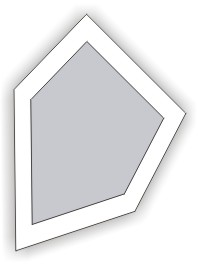
\includegraphics[scale=1]{5.jpg}

Suppose, for convenience, this movement occurs at a rate of one unit in the second coordinate (the time in a way equal to the distance: after a unit of time, each point will overcome the distance equal to one).

During this movement of the polygon will gradually disappear (contact point). Sooner or later, the entire polygon shrinks to a point or a segment, and this time $t$ will be the \textbf{answer to the problem} - the desired radius (and the center of the desired circle will lie in this interval). In fact, if we had to compress the thickness of the polygon $t$ in all directions, and he turned on / segment, then it means that there is a point removed from all sides of the polygon at a distance $t$ And for long distances - a point already exists.

So, we need to learn how to effectively simulate the process of compression. To do this, each side will learn to \textbf{determine the time} after which it will shrink to a point.

For this, consider carefully the process of moving the parties. Note that the vertices of the polygon always move along the bisectors of angles (this follows from the corresponding triangles). But then the question of time, after which the party shrinks, reduces to the question of determining the height of $H$ triangle, which is known for the side length $L$ and two adjacent to the corner of her $\alpha$ and $\beta$. Using, for example, the sine theorem, we get:

$H=L\cdot\frac{\sin\alpha\sin\beta}{\sin(\alpha+\beta)}$ 

Now we can at $O (1)$ determine the time at which the party will shrink to a point.

He brought these times for each side in a \textbf{structure of data to extract a minimum,} for example, a red-black tree($\rm set$ in the language C++).

Now, if we extract the side with the \textbf{least time} \textbf{$H$}, Then the first party will shrink to the point - at the moment $H$. If the polygon has not shrunk to the point / segment, then it should be \textbf{removed} from the side of the polygon, and continue the algorithm for the remaining sides. When you delete a part, we have to \textbf{connect} with each other left and right of her neighbor, \textbf{extending} them to the point where they intersect. It is necessary to find the point of intersection, count the length of two sides and their time of disappearance.

When implemented for each side will have to store number of its right and left neighbor (and thus how to build a doubly linked list of the sides of the polygon). This allows a remote end, and the binding of its two neighbors for $O (1)$.

If you are deleting part is that its side-neighbors \textbf{are parallel,} then it means that the polygon after compression reduces to a point / segment, so we can immediately stop the algorithm and return as a response time of disappearance of the current side (so that problems with parallel sides does not occur).

If such a situation there is no parallel sides, the algorithm will complete before the time at which the polygon will be only two parties - and then the answer to the problem will be the removal of the previous part.

Clearly, the asymptotic behavior of the algorithm is $O (n \log n)$ Because the algorithm consists of $n$ steps, each of which is removed on one side (which is a few transactions $\rm set$ during $O (n \log n)$ ).

\subsection{ Implementation }

We present the implementation of the algorithm described above. This implementation returns the radius of the desired circle, however, the addition of the output of the circle center is not be easy.

This algorithm is elegant because of computational geometry is only required to find the angle between the two sides, the intersection of two lines and two lines on the test parallelism.

Note. It is assumed that applied to the input polygon - \textbf{is strictly convex,} i.e. no three points are collinear.

\begin{verbatim}
const double EPS = 1E-9 ;
const double PI =... ;
 
struct pt {
    double x, y ;
    pt()  { }
    pt(double x, double y): x(x ), y(y) { }
    pt operator -(const pt & p)const {
        return pt(x - p. x, y - p. y);
    }
} ;
 
double dist(const pt & a, const pt & b){
    return sqrt(( a. x - b. x)*(a. x - b. x)+(a. y - b. y)*(a. y - b. y)) ;
}
 
double get_ang(const pt & a, const pt & b){
    double ang = abs(atan2(a. y, a. x)- atan2(b. y, b. x)) ;
    return min(ang, 2 * PI - ang);
}
 
struct line {
    double a, b, c ;
    line(const pt & p, const pt & q){
        a = p. y - q. y ;
        b = q. x - p. x ;
        c = - a * p. x - b * p. y ;
        double z = sqrt(a * a + b * b);
        a / = z, b / = z, c / = z ;
    }
} ;
 
double det(double a, double b, double c, double d){
    return a * d - b * c ;
}
 
pt intersect(const line & n, const line & m){
    double zn = det(n. a, n. b, m. a, m. b);
    return pt (
        - det(n. c, n. b, m. c, m. b)/ zn,
        - det(n. a, n. c, m. a, m. c)/ zn
   );
}
 
bool parallel(const line & n, const line & m){
    return abs(det(n. a, n. b, m. a, m. b)) < EPS ;
}
 
double get_h(const pt & p1, const pt & p2,
    const pt & l1, const pt & l2, const pt & r1, const pt & r2 )
{
    pt q1 = intersect(line(p1, p2 ), line(l1, l2)) ;
    pt q2 = intersect(line(p1, p2 ), line(r1, r2)) ;
    double l = dist(q1, q2);
    double alpha = get_ang(l2 - l1, p2 - p1)/ 2 ;
    double beta = get_ang(r2 - r1, p1 - p2)/ 2 ;
    return l * sin(alpha)* sin(beta)/ sin(alpha + beta);
}
 
struct cmp {
    bool operator()(const pair < double, int > & a, const pair < double, int > & b)const {
        if(abs(a. first - b. first)> EPS )
            return a. first < b. first ;
        return a. second < b. second ;
    }
} ;
 
int main() {
    int n ;
    vector < pt > p ;
    // Read n and p
 
    vector < int > next(n ), prev(n);
    for(int i = 0 ; i < n ; ++ i){
        next[i]=(i + 1)% n ;
        prev[i]=(i - 1 + n)% n ;
    }
 
    set < pair < double, int >, cmp > q ;
    vector < double > h(n);
    for(int i = 0 ; i < n ; ++ i){
        h[i]= get_h (
            p[i], p[next[i]],
            p[i], p[prev[i]],
            p[next[i]], p[next[next[i]] ]
       );
        q. insert(make_pair(h[i], i)) ;
    }
 
    double last_time ;
    while(q. size() > 2){
        last_time = q. begin() - > first ;
        int i = q. begin() - > second ;
        q. erase(q. begin());
 
        next[prev[i]] = next[i];
        prev[next[i]] = prev[i];
        int nxt = next[i],   nxt1 =(nxt + 1)% n,
            prv = prev[i],   prv1 =(prv + 1)% n ;
        if(parallel(line(p[nxt], p[nxt1]), line(p[prv], p[prv1 ])) )
            break ;
 
        q. erase(make_pair(h[nxt], nxt)) ;
        q. erase(make_pair(h[prv], prv)) ;
 
        h[nxt]= get_h (
            p[nxt], p[nxt1],
            p[prv1], p[prv],
            p[next[nxt]], p [(next[nxt]+ 1)% n ]
       );
        h[prv]= get_h (
            p[prv], p[prv1],
            p [(prev[prv]+ 1)% n], p[prev[prv]],
            p[nxt], p[nxt1 ]
       );
 
        q. insert(make_pair(h[nxt], nxt)) ;
        q. insert(make_pair(h[prv], prv)) ;
    }
 
    cout << last_time << endl ;
} 
\end{verbatim}
The main function here - it $get \_h()$ Which, by her side, and the left and right neighbors calculates the disappearance of this side. To do this, search for a point of intersection of the side with the neighbors, and then the above formula is the required calculation time.

\section{ Voronoi diagram in 2D }
\subsection{ Definition }

Dana $n$ points $P_i (x_i, y_i)$ on the plane. Consider the partition of the plane into $n$ areas $V_i$ (Called Voronoi polygons or Voronoi cell, sometimes - polygons proximity cells Dirichlet partition Thyssen), where $V_i$ - The set of all points in the plane that are closer to the point $P_i$ Than all other points $P_k$ :

$V_{i}=\{(x,y):\rho((x,y),P_{i})=\min_{k=1\dots N}\rho((x,y),P_{k})\}$

The very division of the plane is called the Voronoi diagram of a set of points $P_k$.

Here $\rho (p, q)$ - Given metric, this is usually the standard Euclidean metric: $\rho (p, q) = \sqrt {(x_p-x_q) ^ 2 + (y_p-y_q) ^ 2}$ But below will be reviewed and a case of so-called Manhattan metric. Here and below, unless specified otherwise, consider the case of the Euclidean metric

Voronoi cells are convex polygons, some are endless. Points belonging to the definition to several Voronoi cells normally and referred to several cells (in the case of the Euclidean metric the set of points of measure zero, and in the case of the Manhattan metric more complicated than that.)

These polygons were first studied in depth by Voronoi Russian mathematician (1868-1908 gg.).

\subsection{ Properties }

Voronoi diagram is a planar graph, so it has $O (n)$ vertices and edges.
Fix any $i = 1 \ldots n$. Then for each $j = 1 \ldots n, j \ne i$ draw the line - the perpendicular segment $(P_i, P_j)$ And consider that half-plane formed by the straight line, which is a point $P_i$. Then the intersection of all half-planes for each $j$ Voronoi cell will $P_i$.
Each vertex of the Voronoi diagram is the center of a circle drawn through any three points of the set $P$. These circles are essentially used in many of the proofs related to Voronoi diagrams.
Voronoi cell $V_i$ is infinite if and only if the point $P_i$ lies on the boundary of the convex hull of $P_k$.
Consider the graph dual to the Voronoi diagram, i.e. vertices in the graph are the points $P_i$, And the edge is drawn between the points $P_i$ and $P_j$ If their Voronoi cells $V_i$ and $V_j$ have a common edge. Then, provided that no four points lie on a circle, the dual graph of the Voronoi diagram is the Delaunay triangulation (which has many interesting properties).
\subsection{ Application }

Voronoi diagram is a compact data structure that stores all relevant information for a variety of problems of intimacy.

As discussed below, it is the time it takes to build a Voronoi diagram itself, the asymptotic behavior is not considered.

Finding the nearest point for each.
Note the simple fact that if a point $P_i$ is the nearest point $P_j$, This point $P_j$ has "its" in the cell edge $V_i$. It follows that, to find for each point nearest to it, it is enough to see the edges of Voronoi cells. However, each edge belongs to exactly two cells, so it will be seen exactly two times, and due to the linearity of the number of edges we obtain the solution of this problem for $O (n)$.

Finding the convex hull.
Recall that the vertex belongs to the convex hull if and only if its Voronoi cell is infinite. Then we get to the Voronoi diagram any infinite edge, and begin to move in a fixed direction (eg, counter-clockwise) on the cell containing this edge, until we reach the next infinite edge. Then go through this edge to the next cell, and continue to crawl. As a result, viewed edge (but endless) will be sought by the parties of the convex hull. Obviously, the run time - $O (n)$.

Finding the Euclidean minimum spanning tree.
Required to find the minimum spanning tree with vertices at these points $P$ Connecting these points. If we apply the standard graph theory, then, as graph in this case is $O (n ^ 2)$ edges, even the optimal algorithm will have no less asymptotics.

Consider the graph dual Voronoi diagram, i.e. Delaunay triangulation. It can be shown that the presence of the Euclidean minimum spanning tree is equivalent to the construction of the skeleton of the Delaunay triangulation. Indeed, in the Prim algorithm each time matches the shortest edge between two points mozhestvami, if we fix a point of one set, the nearest point to it has an edge in the Voronoi cell, so that the Delaunay triangulation will be present to the nearest point on the edge, as required.

Triangulation is a planar graph, i.e. has a linear number of edges, so we can apply the Kruskal algorithm and an algorithm with a running time $O (n \log n)$.

Finding the largest empty circle.
You want to find the largest radius circle that does not contain any of the points in $P_i$ (The center of the circle must lie inside the convex hull of the points $P_i$ ). Note that, because function of the largest radius of the circle at a given point $f (x, y)$ is strictly monotonic within each Voronoi cell, it attains its maximum at one of the vertices of the Voronoi diagram, or at the point of intersection edges of the diagram and the convex hull (and the number of such points is more than twice the number of edges of the diagram). Thus, we can only go through these points, and for each to find the nearest, i.e. solution for $O (n)$.

\subsection{ Simple algorithm for constructing the Voronoi diagram in $O(n^4)$}

Voronoi diagrams - just a well-studied subject, and for them to get a number of different algorithms for the optimal working asymptotics $O (n \log n)$ And some of these algorithms are even working on average for $O (n)$. However, all of these algorithms are complex.

Consider here the simplest algorithm based on the above properties, each Voronoi cell is the intersection of half-planes. We fix $i$. Spend between point $P_i$ and each point $P_j$ line - the perpendicular, then cross pairs all received direct - we get $O (n ^ 2)$ points, and each check for membership to all $n$ half-planes. As a result, $O (n ^ 3)$ actions we have all the top cell Voronoi $V_i$ (They will not be a more $n$, So we can without compromising asymptotic sort them by the polar angle), and only require the construction of the Voronoi diagram $O (n ^ 4)$ action.

\subsection{ Case of a singular metric }

Consider the following metric:

$\rho (p, q) = \max (| x_p-x_q |, | y_p-y_q |)$

Consideration should start with simple cases - a case of two points $A$ and $B$.

If $A_x = B_x$ or $A_y = B_y$ Then the Voronoi diagram for them to be respectively vertical or horizontal line.

Otherwise, the Voronoi diagram will look like "corner": a segment angle $45$ degrees in the rectangle formed by the points $A$ and $B$, And horizontal / vertical rays of its ends, depending on how long a vertical or a horizontal side of the rectangle.

Special case - when the rectangle is the same length and width, i.e., $| A_x-B_x | = | A_y-B_y |$. In this case, there will be two infinite regions ("corners" formed by two rays parallel to the axes), which by definition must belong to both cells at once. In this case, further defined in the condition, as it should be understood these areas (sometimes artificially introduced a rule that every part relates to his cell).

Thus, even for two points in the Voronoi diagram of the metric is a non-trivial objects, and in the case of a greater number of points of these figures have to be able to quickly cross.

\section{ Finding all faces of a planar graph }
Dan planar stowed in the plane graph $G$ with $n$ vertices. You want to find all the faces. Faces are called part of the plane bounded by edges of the graph.

One of the faces will be different from others in that it will have an infinite area, such a face is called the outer face. In some applications need to find only the outer edge, the algorithm for finding which, as we shall see, in essence no different from the algorithm for all faces.

\subsection{ Euler's theorem }

We present here Euler's theorem and some corollaries from which it follows that the number of edges and faces of a planar simple (no loops or multiple edges) of the graph are of the order $O (n)$.

Let the planar graph $G$ is connected. We denote $n$ the number of vertices in the graph, $m$ - The number of edges $f$ - The number of faces. Then the \textbf{Euler's theorem:}

$f + n - m = 2$

Prove this formula easily follows. In the case of the tree($m = n-1$)Formula is easily verified. If the graph - not a tree, then remove any edge, which belongs to the cycle, with the value $f + n-m$ not change. We repeat this process until you come to a tree, for which the identity $f + n-m = 2$ already installed. Thus, the theorem is proved.
\textbf{Corollary.} For any planar graph let $k$ - The number of connected components. Then we have:

$f + n - m = 1 + k$

\textbf{Corollary.} The number of edges $m$ simple planar graph is of the $O (n)$.

Proof. Let the graph $G$ is connected and $n \ge 3$ (In the case $n <3$ approval is obtained automatically.) Then, on the one hand, each face is bounded by at least three edges. On the other hand, each edge is limited to a maximum two faces. Consequently, the $3f \le 2m$ Whence, substituting this into Euler's formula, we get:

$f+n-m=2\Leftrightarrow3f=6-3n+3m\Leftrightarrow6-3n+3m\leq2m\Leftrightarrow m\leq3n-6$

i.e. $m = O (n)$.
If the graph is not connected, then summing the estimates for its connected components, we again obtain $m = O (n)$, As required.

\textbf{Corollary.} The number of faces $f$ simple planar graph is of the $O (n)$.

This follows from the previous investigation and communication $f = 2 - n + m$.

\subsection{ Bypassing all facets }

Always assume that the graph, if it is not connected, laid on the plane so that no connected component is not contained within the other (for example, a square with lying strictly inside the segment - an incorrect test for our algorithm).

Of course, it is assumed that the graph is well laid on a plane, that no two vertices are not the same, and the edges do not intersect in "unauthorized" places. If the input graph admits such intersecting edges, then a pre-need to get rid of them, entering into every intersection additional vertex (it should be noted that as a result of this process rather than $n$ points we can get about $n ^ 2$ points). For more on this process, see below in the appropriate section.

Let each vertex all outgoing edges from it in order of the polar angle. If it is not, then they should be streamlined, making the sort of each adjacency list (as $m = O (n)$, It will take $O (n \log n)$ operations).

Now choose an arbitrary edge $(A, b)$ And let the next round. Coming to some vertex $v$ on an edge, out of this summit we have to for the next edge in the sort order.

For example, in the first step, we are in the top $b$ And the need to find the top $a$ at the top of the list of adjacency $b$, Then we denote $c$ next vertex in the adjacency list (if $a$ was the latter, as $c$ take the first vertex), and walk along the edge $(B, c)$.

By repeating this process many times, we will sooner or later come back to the starting edge $(A, b)$ And then have to stop. It is easy to see that with such a circuit we will do exactly one edge. And the direction of the circuit will be counter-clockwise to the outer edge, and clockwise - for internal faces. In other words, in such a circuit inside edge will always be on the right side of the current edge.

So we learned how to do one face, starting from any edge on its boundary. Learn to choose the starting left edges so that the resulting faces are not repeated. Note that each edge of two different ways in which it can be traversed: each of them will get their faces. On the other hand, it is clear that one is oriented edge belongs to exactly one face. Thus, if we are going to mark all the edges of each detected face in a array $\rm used$ And do not run out of bypass already marked edges, then we will do all the faces (including foreign), even just once.

Present directly \textbf{implementing} this workaround. We assume that the graph $G$ the adjacency lists is arranged in the corner, and multiple edges and loops are not available.

The first embodiment of a simplified, the next vertex in the adjacency list it looks simple search. Such an implementation of theoretical work $O (n ^ 2)$, Although in practice many tests, it works very fast (with a hidden constant, much smaller than unity).

\begin{verbatim}
int n ; // Number of vertices
vector < vector < int > > g ; // Graph
 
vector < vector < char > > used(n);
for(int i = 0 ; i < n ; ++ i )
    used[i].resize(g[i].size());
for(int i = 0 ; i < n ; ++ i )
    for(size_t j = 0 ; j < g[i].size() ; ++ j )
        if(! used[i ][ j ]){
            used[i ][ j]= true ;
            int v = g[i ][ j],  pv = i ;
            vector < int > facet ;
            for(;;){
                facet. push_back(v);
                vector < int >::iterator it = find(g[v].begin(), g[v].end(), pv);
                if(++ it == g[v].end()) it = g[v].begin() ;
                if(used[v ][ it - g[v].begin() ]) break ;
                used[v ][ it - g[v].begin()]= true ;
                pv = v,  v = * it ;
            }
            ... output facet - the current face...
        } 
\end{verbatim}
Another, more optimized version of the implementation - enjoys the fact that the top on the list in order of adjacency corner. If you implement the function $\rm cmp \_ang$ Comparison of two points over the polar angle relative to the third point (for example, arrange it in a class, as in the example below), the search terms in the list of adjacency can use binary search. The result is the realization of $O (n \log n)$.

\begin{verbatim}
class cmp_ang {
    int center ;
public :
    cmp_ang(int center): center(center )
        { }
    bool operator()(int a, int b)const {
        ... should return true, if the point is a
        b less than the polar angle relative to center...
    }
} ;
 
 
int n ; // Number of vertices
vector < vector < int > > g ; // Graph
 
vector < vector < char > > used(n);
for(int i = 0 ; i < n ; ++ i )
    used[i].resize(g[i].size());
for(int i = 0 ; i < n ; ++ i )
    for(size_t j = 0 ; j < g[i].size() ; ++ j )
        if(! used[i ][ j ]){
            used[i ][ j]= true ;
            int v = g[i ][ j],  pv = i ;
            vector < int > facet ;
            for(;;){
                facet. push_back(v);
                vector < int >::iterator it = lower_bound(g[v].begin(), g[v].end(),
                    pv, cmp_ang(v)) ;
                if(++ it == g[v].end()) it = g[v].begin() ;
                if(used[v ][ it - g[v].begin() ]) break ;
                used[v ][ it - g[v].begin()]= true ;
                pv = v,  v = * it ;
            }
            Count... output facet - the current face...
        } 
\end{verbatim}
And possible option, based on the container $map$, Because we only need to quickly know the position numbers in the array. Of course, such an implementation would also work $O (n \log n)$.

It should be noted that the algorithm does not work correctly with \textbf{isolated} peaks - such peaks it just does not show up as individual faces, though, from a mathematical point of view, they must be a single connected component and faces.

In addition, a special face is the \textbf{outer face.} How to distinguish it from the "normal" faces, described in the next section. Note that if the graph is not connected, the outer face is composed of several units, each of these circuits will be found by the algorithm separately.

\subsection{ Isolation of the outer edge }

The above code displays all the faces, making no distinction between the outer and inner faces of the edge. In practice, on the contrary, you want to find, or just the outer edge, or just internal. There are several methods of allocating the outer edge.

For example, you can define the area - outside face must have the largest area (it should only take into account that the inner face can have the same area as the outside). This method will not work if the planar graph $G$ is not connected.

Another, more reliable criterion - towards crawling. As noted above, all of the faces except the external cost in the clockwise direction. Outer edge, even if it consists of several circuits to cost algorithm counterclockwise. Determine the direction of the circuit by simply considering the symbolic area of the polygon. The area can be considered right along the inner loop. However, this method has its subtlety - processing faces of zero area. For example, if the graph is a single edge, then the algorithm will find a unique edge, the area of ​​which is zero. Apparently, if a face has zero area, it is the outer edge.

In some cases, it applies such criteria as the number of vertices. For example, if the graph is a convex polygon with conducted in it non-intersecting diagonals, its outer edge will contain all vertices. But again, you have to be careful with the case where both the outer and inner faces have the same number of vertices.

Finally, there are the following method to find the outer edge: you can start from such a special edge that was found in the outer face will result. For example, you can take the left-most vertex (if there are several, that will suit any) and select the edge of it, coming first in the sort order. As a result of bypassing this edge will face the outside. This method can be extended to the case of a disconnected graph: the need in each component to find the top of the left and run circumvention of the first edge of it.

We present a simple implementation of the method based on the sign area (myself bypassing I took as an example $O (n ^ 2)$ Here it does not matter). If the graph is not connected, the code "... the external face is..." made separately for each circuit component of the external face.

\begin{verbatim}
       ... normal code to detect faces...
       ... immediately after the loop, detecting another side:...
         
        // Find the area
        double area = 0;
        // Add a dummy point for ease of calculation of the area
        facet. push_back(facet[0 ]);
        for(size_t k = 0 ; k + 1 < facet. size() ; ++ k )
            area + =(p[facet[k]]. first + p[facet[k + 1]]. first )
                *(p[facet[k]]. second - p[facet[k + 1]]. second);
        if(area < EPS )
         ... face is a foreign...
    } 
\end{verbatim}
\subsection{ The construction of a planar graph }

For the above algorithms is essential that the input graph is a well-packed planar graph. However, in practice it is often fed to the input of a set of program segments, possibly overlapping with each other in "unauthorized" places, and to build on these segments of a planar graph.

Implement the construction of a planar graph in the following way. We fix any input segment. Now this cross section with all the other sections. These points of intersection, and the ends of the segment set in a vector, and its sort in the standard way (i.e. first one coordinate, with equal - on the other). Then go through this vector and will add an edge between adjacent points in this vector (of course, making sure that we have not added the loop). Carrying out this process for all segments, i.e. for $O (n ^ 2 \log n)$ We construct the corresponding planar graph (which will be $O (n ^ 2)$ points).

Implementation:

\begin{verbatim}
const double EPS = 1E-9 ;
 
struct point {
    double x, y ;
    bool operator <(const point & p)const {
        return x < p. x - EPS || abs(x - p. x)< EPS && y < p. y - EPS ;
    }
} ;
 
map < point, int > ids ;
vector < point > p ;
vector < vector < int > > g ;
 
int get_point_id(point pt){
    if(! ids. count(pt)) {
        ids[pt]=(int)p. size() ;
        p. push_back(pt);
        g. resize(g. size() + 1);
    }
    return ids[p];
}
 
void intersect(pair < point,point > a, pair < point,point > b, vector < point > & res){
   //standard procedure, crosses two segments a and b, and throws the result in res
   //if the segments overlap, then throws those ends that get inside the first segment
}
 
int main() {
    int m ;
    vector < pair < point,point > > a(m);
    // reading
 
    // Build the graph
    for(int i = 0 ; i < m ; ++ i){
        vector < point > cur ;
        for(int j = 0 ; j < m ; ++ j )
            intersect(a[i], a[j], cur);
        sort(cur. begin(), cur. end());
        for(size_t j = 0 ; j + 1 < cur. size() ; ++ j){
            int x = get_id(cur[j]),  y = get_id(cur[j + 1 ]);
            if(x ! = y){
                g[x].push_back(y);
                g[y].push_back(x);
            }
        }
    }
    int n =(int)g. size() ;
    // Sort of angle and removal of multiple edges
    for(int i = 0 ; i < n ; ++ i){
        sort(g[i].begin(), g[i].end(), cmp_ang(i)) ;
        g[i].erase(unique(g[i].begin(), g[i].end() ), g[i].end());
    }
} 
\end{verbatim}
\section{ Closest pair of points }
\subsection{ Statement of the problem }

Dana $n$ points $p_i$ on the plane defined by its coordinates $(X_i, y_i)$. Need to find one such two points, the distance between them is minimal:

$\min_{i,j=0\dots n-1,i\neq j}\rho(p_{i},p_{j})$

Distance we take the usual Euclidean:

$\rho(p_{i},p_{j})=\sqrt{(x_{i}-x_{j})^{2}+(y_{i}-y_{j})^{2}}$

Trivial algorithm - through all the pairs and calculate the distance of each - works for $O (n ^ 2)$. The following is an algorithm that runs in time $O (n \log n)$. This algorithm was proposed DRUGS (Preparata) in 1975, Drug and Shamos also show that the decision tree model, this algorithm is asymptotically optimal.

\subsection{ Algorithm }

We construct an algorithm for the general scheme of algorithms \textbf{"divide-and-rule":} the algorithm is made ​​out as a recursive function, which is passed a set of points, this recursive function splits the set in half, calling itself recursively on each half, and then performs some actions to integrate answers. Merge operation is to detect when a single point of optimal solutions lie at the half, and the other point - to another (in this case a recursive call on each half separately to find the pair, of course, can not.) The main difficulty, as always, lies in the effective implementation of this stage of the association. If a recursive function is passed a set of $n$ points, the stage union should work no more than $O (n)$ Then the asymptotic behavior of the algorithm $T (n)$ will be out of the equation:

$T (n) = 2 T (n / 2) + O (n).$

The solution of this equation is known to be $T (n) = O (n \log n)$.

So, proceed to the construction of the algorithm. In the future to come to the effective implementation of the steps of combining, breaking a lot of points on the two according to their will $x$ -Coordinates: in fact we spend some vertical line which divides the set of points into two subsets of approximately equal size. Such a division is convenient to read as follows: sort the points of the standard as a pair of numbers, that is:

$p_{i}<p_{j}\Leftrightarrow(x_{i}<x_{j})\vee\left((x_{i}=x_{j})\wedge(y_{i}<y_{j})\right)$

Then we take the average, after sorting point $p_m$($m = \lfloor n / 2 \rfloor$ ), All point to it and very $p_m$ belongs to the first half, and all points after it - in the second half:

$A_1 = \{p_i \| i = 0 \ldots m \},$

$A_2 = \{p_i \| i = m +1 \ldots n-1 \}.$

Now called recursively on each of the sets $A_1$ and $A_2$ We'll find the answers $h_1$ and $h_2$ for each half. Take the best of them: $h = \min (h_1, h_2)$.

Now we need to make \textbf{the stage union,} i.e. try to find such a pair of points, the distance between them is less than $h$, And one point is in the $A_1$ And the other - in $A_2$. Obviously, it is sufficient to consider only those points which are separated by a vertical line section is not a distance less than $h$ i.e. many $B$ considered at this stage of points is:

$B = \{p_i \| \| x_i - x_m | <h \}.$

For each point of the set $B$ we must try to find the points that are closer to it than $h$. For example, it suffices to consider only those points, the coordinate $y$ which differ by no more than $h$. Moreover, it makes no sense to consider the points that have $y$ Coordinate more $y$ Coordinates of the current point. Thus, for each point $p_i$ define the set of points under consideration $C (p_i)$ as follows:

$C(p_{i})=\{p_{j}|p_{j}\in B,y_{i}-h<y_{j}\leq y_{i}\}$

If we sort the points of $B$ on $y$ Coordinate, then find $C (p_i)$ it will be very easy: a few points in a row to the point $p_i$.

So, in the new notation \textbf{stage association} is as follows: to construct a set $B$ And sort it according to terms $y$ Coordinate, then for each point $p_i \in B$ consider all points $p_j \in C (p_i)$ And each pair $(P_i, p_j)$ calculate the distance and compare with the current best distance.

At first glance, it is still sub-optimal algorithm: it seems that the size of the sets $C (p_i)$ be of the order $n$ And the required asymptotic behavior does not work. However, surprisingly, it can be shown that the size of each of the sets $C (p_i)$ is the value $O (1)$ i.e. does not exceed a small constant, regardless of the points themselves. The proof is given in the next section.

Finally, we turn our attention to the sort of which the above algorithm contains just two: first sorting the pairs($x$, $y$)And then sort the elements of $B$ on $y$. In fact, both of these sorts inside a recursive function, you can get rid of (or we would not have achieved evaluation $O (n)$ for the stage of association, and the general asymptotic algorithm would have been $O (n \log ^ 2 n)$ ). Get rid of the first sort is easy - just in advance, before the launch of recursion to perform this sort: for recurrence within the elements themselves do not change, so there is no need to sort again. With the second sorting little harder to fulfill its pre-fail. But, remembering the \textbf{mergesort} (merge sort), which also works on the principle of divide-and-conquer, you can simply embed this sort in our recursion. Let recursion, taking a set of points (as we recall, ordered in pairs $(X, y)$)Returns the same set, but already sorted coordinate $y$. For this, simply merge (for $O (n)$)Two results returned by the recursive call. Thus a sorted by $y$ many.

\subsection{ Asymptotic evaluation }

To show that the above algorithm is indeed running for $O (n \log n)$ It remains to prove the following fact: $| C (p_i) | = O (1)$.

So, let us consider some point $p_i$ We recall that many $C (p_i)$ - The set of points $y$ -Coordinate is no more $y_i$, But not less $y_i-h$ And, in addition, the coordinate $x$ and the point itself $p_i$ And all the points $C (p_i)$ lie in a strip $2h$. In other words, the point under consideration $p_i$ and $C (p_i)$ lie in the size of the rectangle $2h \times h$.

Our task - to estimate the maximum number of points that may lie in the rectangle $2h \times h$, Thus we estimate and the maximum size of the set $C (p_i)$ (It will be one less, because in this rectangle is also a point $p_i$ ). It should not be forgotten that, in general, can meet and duplicate points.

Recall that $h$ was obtained from at least two of the results of recursive calls - from sets $A_1$ and $A_2$, And $A_1$ contains points to the left of the line section and partially in it, $A_2$ - The remaining section of a line and a point on its right. For any pair of points $A_1$, As well as from $A_2$, The distance can not be less than $h$ - Otherwise it meant incorrectness recursive function.

For the maximum number of points in the rectangle $2h \times h$ divide it into two squares $h \times h$, To the first point of the square consists of all $C (p_i) \cap A_1$, And the second - all the others, i.e. $C (p_i) \cap A_2$. From the above considerations, it follows that each of the boxes to the distance between any two points is at most $h$. But then, this means that in each square to four points!

Indeed, suppose that there is a square $h \times h$ And the distance between any two points is at most the same $h$. We prove that the square can not be more than 4 points. For example, this can be done as follows: we divide this square into 4 squares with sides $h / 2$. Then in each of these small squares can not be more than one point (because even diagonal equal $h / \sqrt {2}$, Which is less $h$ ). Consequently, all the square can not be more than 4 points.

Thus we have proved that in the rectangle $2h \times h$ can not be more $4 \cdot 2 = 8$ points, and thus the size of the set $C (p_i)$ can not exceed $7$, As required.

\subsection{ Implementation }

We introduce a data structure for storing point (its coordinates and a number) and comparison operators are needed for the two types of order:

\begin{verbatim}
struct pt {
    int x, y, id ;
} ;
 
inline bool cmp_x(const pt & a, const pt & b){
    return a. x < b. x || a. x == b. x && a. y < b. y ;
}
 
inline bool cmp_y(const pt & a, const pt & b){
    return a. y < b. y ;
}
 
pt a[MAXN]; 
\end{verbatim}
For easy implementation of recursion, we introduce the auxiliary function $upd \_ans()$ Which will calculate the distance between two points, and check whether it is not better than the current response:

\begin{verbatim}
double mindist ;
int ansa, ansb ;
 
inline void upd_ans(const pt & a, const pt & b){
    double dist = sqrt(( a. x - b. x)*(a. x - b. x)+(a. y - b. y)*(a. y - b. y)+.0);
    if(dist < mindist )
        mindist = dist,  ansa = a. id,  ansb = b. id ;
} 
\end{verbatim}
Finally, the implementation itself recursively. It is assumed that the array before calling $a []$ already sorted by $x$ -Coordinate. Recursion is simply passed two pointers $l$, $r$ Which indicate that it should search for the answer to $a [l \ldots r]$. If the distance between $r$ and $l$ too small, the recursion must stop and perform trivial algorithm to scan for the nearest pair and then sort on the subarray $y$ -Coordinate.

To merge two sets of points obtained by recursive calls, one (ordered by $y$ Coordinate), we use a standard feature STL $merge()$ And create a secondary buffer $t []$ (One for all recursive calls). (Use $inplace \_merge()$ impractical, because it generally does not work in linear time).

Finally, the set $B$ stored in the same array $t$.

\begin{verbatim}
void rec(int l, int r){
    if(r - l <= 3){
        for(int i = l ; i <= r ; ++ i )
            for(int j = i + 1 ; j <= r ; ++ j )
                upd_ans(a[i], a[j ]);
        sort(a + l, a + r + 1, & cmp_y);
        return ;
    }
 
    int m =(l + r)>> 1 ;
    int midx = a[m].x ;
    rec(l, m ),  rec(m + 1, r);
    static pt t[MAXN];
    merge(a + l, a + m + 1, a + m + 1, a + r + 1, t, & cmp_y);
    copy(t, t + r - l + 1, a + l);
 
    int tsz = 0 ;
    for(int i = l ; i <= r ; ++ i )
        if(abs(a[i].x - midx)< mindist){
            for(int j = tsz - 1 ; j >= 0 && a[i].y - t[j].y < mindist ; -- j )
                upd_ans(a[i], t[j ]);
            t[tsz ++]= a[i];
        }
} 
\end{verbatim}
By the way, if all the coordinates are integers, for the duration of recursion can never go to fractional quantities, and store in $mindist$ square minimum distance.

In the main program call the recursion as follows:

\begin{verbatim}
sort(a, a + n, & cmp_x);
mindist = 1E20 ;
rec(0, n - 1); 
\end{verbatim}
\subsection{ Summary: Search the triangle with minimum perimeter }

The algorithm described above is interesting generalized to the problem: given a set of points to choose three different points so that the sum of pairwise distances between them was minimal.

In fact, to solve this problem the algorithm is the same: we divide the field into two halves of the vertical line, call the recursive solution of two halves, select the minimum $minper$ perimeters of the found, build a strip thickness $minper / 2$, And it sort out all the triangles, which may improve the response. (Note that a triangle with a perimeter $\le minper$ the long side $\le minper / 2$.)

\subsection{ Tasks in the online judges }

List of tasks that can be reduced to search the next two points:

UVA 10245 \textbf{"The Closest Pair Problem"} [Difficulty: Easy]

SPOJ 8725 CLOPPAIR \textbf{"Closest Point Pair"} [Difficulty: Easy]

CODEFORCES Saratov Team Olympiad - 2011 \textbf{"Minimum"} [Difficulty: Medium]

Google CodeJam 2009 Final \textbf{"Min Perimeter"} [Difficulty: Medium]

SPOJ 7029 CLOSEST \textbf{"Closest Triple"} [Difficulty: Medium]

\section{ Geometric transformation of inversion }
Geometric transformation of inversion (inversive geometry) - a special type of transformation points on the plane. The practical benefit of this transformation is that it often allows one to reduce the solution of the geometric problem \textbf{with circles} to the solution of the corresponding problem \textbf{with straight,} which usually has a much simpler solution.

Apparently, the founder of this field of mathematics was Ludwig Immanuel Magnus (Ludwig Immanuel Magnus), who in 1831 published an article on the inverse transformations.

\subsection{ Definition }

Fix a circle with center $O$ radius $r$. Then the \textbf{inversion} point $P$ on this circle is called a point $P ^ \prime$ Which lies on the line $OP$, And the distance satisfies the condition:

$OP \cdot OP ^ \prime = r ^ 2.$

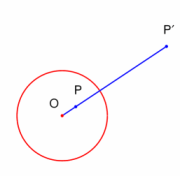
\includegraphics[scale=0.75]{6.png}

If we assume that the center $O$ circle is at the origin, we can say that the point $P ^ \prime$ has the same polar angle as $P$, And the distance is calculated from the above formula.

In terms \textbf{of complex numbers,} the inversion transformation is expressed quite simply, if we assume that the center $O$ circle is at the origin:

$z ^ \prime = r ^ 2 \cdot \frac {z} {| z | ^ 2}.$

With the dual element $\overline {z}$ You can get a simple form:

$z ^ \prime = \frac {r ^ 2} {\overline {z}}.$

Application of inversion (at mid-board) to the image of chess board provides an interesting picture (right):

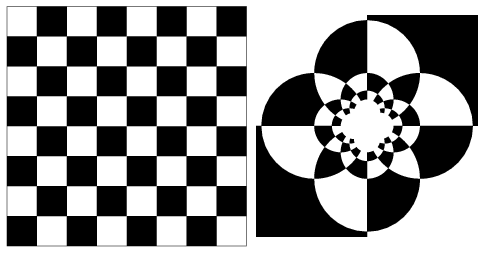
\includegraphics[scale=0.5]{7.png}

\subsection{ Properties }

Clearly, any point \textbf{on the circle,} which is made ​​with respect to the inversion transformation, the mapping goes to for themselves. Any point \textbf{inside} the circle goes to the \textbf{outside} area, and vice versa. It is believed that the center of the circle goes to a point of "infinity" $\infty$ And the point of "infinity" - on the contrary, in the center of the circle:

$(O) ^ \prime = \infty,$
$(\infty) ^ \prime = O.$

Obviously, the repeated use of the inversion transformation \textbf{draws} its first application - all the points come back:

$\left (P ^ \prime \right) ^ \prime \equiv P.$

\subsubsection{ Generalized circle }

Generalized circle - either a circle or a straight line (it is believed that this is also a circle, but with an infinite radius).

Key property of the inversion transformation - which when applied generalized circle \textbf{always translate into a generalized circle} (assuming the conversion of pointwise inversion applied to all points in the figure).

Now we'll see what's going on with straight lines and circles under the inversion transformation.

\subsubsection{ Inversion of the line passing through the point O}

States that any straight line passing through $O$ After the inversion transformation \textbf{does not change.}

In fact, any point on this line, except $O$ and $\infty$, Goes by definition also a point of the line (and in the end we got a point fill the entire line as a whole, because the transformation is reversible inversion). The remaining points $O$ and $\infty$ But the inversion they pass each other, so the proof is completed.

\subsubsection{ Inversion of the line not passing through the point O}

Argued that any such move straight \textbf{into the circle} passing through $O$.

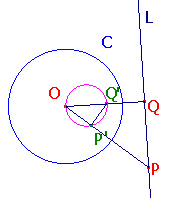
\includegraphics[scale=0.5]{8.png}

Consider any point $P$ this line, and we also consider the point $Q$ - Closest to $O$ point of the line. It is clear that the segment $OQ$ perpendicular to the line, so they formed an angle $\angle PQO$ - Direct.

We now use \textbf{Lemma of equal angles,} which we prove later, this lemma gives us the equation:

$\angle PQO = \angle Q ^ \prime P ^ \prime O.$

Therefore, the angle $\angle Q ^ \prime P ^ \prime O$ too straight. Because we take a point $P$ all, it turns out that the point $P ^ \prime$ lies on the circle, built on $O Q ^ \prime$ as diameter. It is easy to understand that in the end, all points on the line will cover the whole circumference of the whole, therefore, we are done.

\subsubsection{ Inversion of a circle passing through the point O}

Any such circle becomes \textbf{a straight line} not passing through the point $O$.

Indeed, this follows immediately from the previous point, if we think of the reversibility inversion transformation.

\subsubsection{ Inversion of a circle not passing through O}

Any such move \textbf{in} a circle \textbf{a circle,} are still passing through $O$.

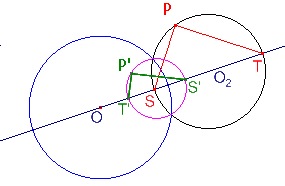
\includegraphics[scale=0.5]{9.png}

Indeed, consider any such circle $Z$ with center $O_2$. Connect the center $O$ and $O_2$ circles straight: this line hits the circle $Z$ at two points $S$ and $T$ (Obviously, $ST$ - Diameter $Z$ ).

Now consider any point $P$ Lying on the circle $Z$. Angle $\angle SPT$ line for any such point, but the corollary of \textbf{Lemma on equal angles} to be as direct and angle $\angle S ^ \prime P ^ \prime T ^ \prime$, Which implies that the point $P ^ \prime$ lies on the circle, built on the segment $S ^ \prime T ^ \prime$ as diameter. Again, it is easy to understand that all images $P ^ \prime$ eventually cover this circle.

Clearly, this new circle can not pass through $O$ : Otherwise the point $\infty$ would have to belong to the old circle.

\subsubsection{ Lemma about equal angles }

This accessory is a property that was used above in the analysis of the transformation of inversion.

Formulation
Consider two points $P$ and $Q$ And apply to them the inversion transformation, we get the point $P ^ \prime$ and $Q ^ \prime$. Then the following angles are equal:

$\angle PQO = \angle Q ^ \prime P ^ \prime O,$

$\angle QPO = \angle P ^ \prime Q ^ \prime O.$

Proof
Prove that the triangle $\triangle PQO$ and $\triangle Q ^ \prime P ^ \prime O$ similar (order of vertices is important!).

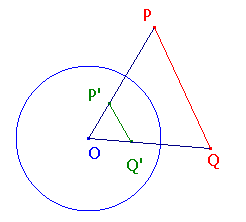
\includegraphics[scale=0.5]{10.png}

In fact, by the definition of the inversion transformation we have:

$OP \cdot OP ^ \prime = r ^ 2,$

$OQ \cdot OQ ^ \prime = r ^ 2,$

from which we obtain:

$OP \cdot OP ^ \prime = OQ \cdot OQ ^ \prime,$

$\frac{OP}{OQ}=\frac{OQ'}{OP'}$

Thus, the triangles $\triangle PQO$ and $\triangle Q ^ \prime P ^ \prime O$ have a common angle, and the two adjacent sides are proportional to it, therefore, the triangles are similar, and therefore the corresponding angles are equal.

Consequence of Lemma
If there are any three points $P$, $Q$, $R$, The point $R$ lies in the interval $OQ$, It holds:

$\angle QPR = \angle Q ^ \prime P ^ \prime R ^ \prime,$

and these angles are oriented in different directions (i.e., if we consider these two corners as directed, they are of opposite sign).

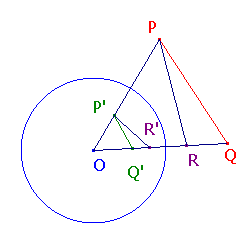
\includegraphics[scale=0.5]{11.png}

For proof, note that $\angle QPR$ - Is the difference of two angles $\angle QPO$ and $\angle RPO$, Each of which can apply Lemma Equal angles:

$\angle QPR=\angle QPO-\angle RPO=\angle P'Q'O-\angle P'R'o=\angle R'P'Q'=\angle Q'P'R'$

In the implementation of the last transition, we have changed the order of the points, which means that we have changed the orientation of the corner to the opposite.

\subsubsection{ Conformality }

Inversion transformation is conformal, that \textbf{preserves the angles at the points of intersection.} In this case, if the angles seen as oriented, the orientation angles of the application of the inversion is reversed.

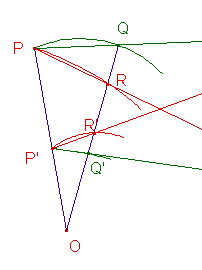
\includegraphics[scale=0.5]{12.png}

To \textbf{prove} this, consider any two curves intersect at the $P$ and having in her tangents. Let the first point of the curve will go $Q$, Second - a point $R$ (Which we rushed to the limit to $P$ ).

Obviously, after the reversal of the curves will continue to overlap (of course, if they do not pass through the point $O$, But that we will not be), and the point of intersection will be $P ^ \prime$.

Given that the point $R$ lies on the line joining $O$ and $Q$, We see that we can apply the corollary of Lemma on equal angles from which we obtain:

$\angle QPR=-\angle Q'P'R'$

where under the "minus" we mean that the corners are oriented in different directions.

Letting point $Q$ and $R$ to the point $P$ We in the limit that equality - an expression of the angle between the intersecting curves, as required.

\subsubsection{ Property of reflection }

If $M$ - Generalized circle, then the transformation of inversion, it is \textbf{stored} and then only when $M$ \textbf{orthogonal to the} circle $C$ About which is inverse($M$ and $C$ considered to be different.)

The proof of this property is interesting because it \textbf{demonstrates the} use of the geometric inversion to avoid the circles, and the task.

The first step in \textbf{the proof} will be an indication of the fact that $M$ and $C$ have at least two points of intersection. In fact, the transformation of inversion $C$ maps the interior of the circle in her appearance, and vice versa. Time $M$ after the conversion has not changed, that means it contains points from both the inside and from the exterior of the circle $C$. It follows that the points of intersection of the two (the one it can not be - it means touching the two circles, but in this case, obviously, be the condition can not, be the same circle also can not by definition).

Denote a point of intersection in $A$, The other - a $B$. Consider a circle with center $A$, And convert it inversion. Note that if and circle $C$ And generalized circle $M$ should become the intersecting lines. Given the inverse conformal transformation, we find that $M$ and $M ^ \prime$ same if and only if the angle between the two intersecting straight lines (in fact, the first cast inversion - a relatively $C$ - Changes the direction of the angle between the circles to the opposite, so if the circle is its own inverse, the angles between the intersecting lines on both sides should be the same, and equal $\frac {180} {2} = 90$ degrees).

\subsection{ Practical application }

It is worth noting that the application must be considered in the calculation of a large \textbf{error} introduced by the transformation of inversion may appear very small fractions of orders, and is usually due to high error inversion method works well only with relatively small coordinates.

\subsubsection{ Constructing shapes after inversion }

In the software calculations are often more convenient and safe to use not ready formulas for the coordinates and radii of the resulting generalized circles, and restore every time straight / circle at two points. If the recovery is sufficient to take direct any two points and calculate their images and connect the line, then the circles is more complicated.

If we want to find a circle, resulting in a direct inversion, according to the above calculations, it is necessary to find the nearest point to the center of inversion $Q$ line to apply the inversion (getting a certain point $Q ^ \prime$ ), And then the desired circle will have a diameter of $O Q ^ \prime$.

Now suppose that we want to find a circle, resulting in a different inversion circle. Generally speaking, the center of the new circle - does not coincide with the image of the old center of the circle. To determine the center of the new circle can take this concept: to push through the inversion center and the center of the circle of the old line, see its point of intersection with the old circle - let it be a point $S$ and $T$. Segment $ST$ the diameter of the circle of the old forms, and easy to understand that after the inversion this segment will continue to form the diameter. Consequently, the center of the new circle can be found as the average points $S ^ \prime$ and $T ^ \prime$.

\subsubsection{ Parameters of the circle after inversion }

Required for a given circle (the known coordinates of its center $(X_0, y_0)$ and radius $r_0$)To determine in advance which it enters the circle after conversion inversion circle with center $(X_c, y_c)$ and radius $r$.

i.e. we solve the problem described in the previous paragraph, but we want to get a solution in closed form.

The answer appears in the form of formulas:

$x ^ \prime = x_c + s (x_0 - x_c),$
$y ^ \prime = y_c + s (y_0 - y_c),$
$r ^ \prime = | s | \cdot r_0,$

where

$s=\frac{r^{2}}{(x_{0}-x_{c})^{2}+(y_{0}-y_{c})^{2}-r_{0}^{2}}$

Mnemonic, these formulas can be remembered as: center of the circle goes to "almost" as to transform inversion, only the denominator in addition $| Z | ^ 2 = (x_0 - x_c) ^ 2 + (y_0 - y_c) ^ 2$ have yet subtrahend $r_0 ^ 2$.

These formulas are derived exactly as described in the preceding paragraph algorithm: find an expression for the two diametrical points $S$ and $T$ Then applied to them, inversion, and then the arithmetic mean of their coordinates. Similarly, we can calculate the radius as half the length of the segment $ST$.

\subsubsection{ Application: the partition problem points on the circle }

Dana $2n$ different points on the plane, and any point $O$ Different from all the rest. Prove that there is a circle passing through the point $O$ Such that the inside and outside of it will be based on the same number of points of the set, i.e., on $n$ pieces.

For the \textbf{proof} we make the transformation inversion selected point $O$ (With any radius, for example, $r = 1$ ). Then the desired circle will fit straight line does not pass through the point $O$. And on one side of the line is a half-plane corresponding to the inner circle, and on the other - the corresponding appearance. It is clear that there is always a line which divides the set of $2n$ points in half by $n$ points, and it does not pass through the point $O$ (For example, a straight line can be obtained by turning the whole picture at any angle such that nor in any of the considered $2n +1$ points do not match the coordinates $x$ And then just taking a vertical line between $n$ Th and $n +1$ Nd points). This line corresponds to the desired circle passing through the point $O$ And hence the assertion.

\subsubsection{ Usage to solve problems in computational geometry }

A remarkable property of geometric inversion - that in many cases it can simplify the task set by the geometric, consider replacing only the circles of direct examination.

i.e. if the task is not a straightforward operation with various circles, it makes sense to apply to the input data inversion transformation, try to solve the problem without obtaining modified circles (or a smaller number of them), and then re-use inversion to obtain the solution of the original problem.

An example of this problem is described in the next section.

\subsubsection{ Steiner chain }

Given two circles $C$ and $D$ One is located in the interior of the other. Then draw a third circle $E$ Relating to these two circles, and then starts an iterative process: each time you draw a new circle so that it \textbf{touches the} previous draw, and the first two. Sooner or later, another draw a circle intersect with some of the already delivered, or at least to touch her.

Case of the intersection:

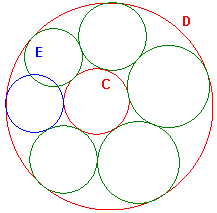
\includegraphics[scale=0.5]{13.png}

If you touch:

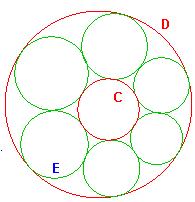
\includegraphics[scale=0.5]{14.png}

Accordingly, our task - to put \textbf{as many} of the circles so that the intersection (i.e., the first of the cases) were not. The first two circles (external and internal) are fixed, we can only vary the position of the first concerns of the circle, then everything on the circle put one.

If you touch the receiving chain of circles is called \textbf{a Steiner chain.}

With this so-called chain of linked \textbf{approval Steiner} (Steiner's porism): if there is at least one chain Steiner (i.e., there is a provision regarding the start of the circle, leading to a chain of Steiner), for any other choice of starting tangent circles will get the chain Steiner, and the number of circles in it will be the same.

From this statement it follows that the solution to maximize the number of circles the answer is independent of the position of the first set of the circle.

\textbf{Proof} and constructive algorithm for the following. Note that the problem has a simple solution in the case when the centers of the outer and inner circles coincide. Clearly, in this case the number of circles set does not depend on the first set. In this case, all the circles have the same radius and the number of centers and coordinates can be calculated by simple formulas.

To go to this simple situation of any supply to the input, apply the transformation of inversion with respect to a circle. We need to center the inner circle moved and coincided with the center of the outer, so look for a point with respect to which we take the inversion, it is only necessary on the line connecting the centers of the circles. Using the formulas for the coordinates of the center of the circle after applying inversion, can equate to the center of inversion, and to solve this equation. Thus, we are of arbitrary situation can go to a simple, symmetric case, and by solving the problem for him, re-apply the inversion transformation and obtain the solution of the original problem.

\subsubsection{ Technological applications: direct Lipkin-Settling }

For a long time the problem of transforming circular (rotational) motion into linear remained very challenging in engineering, managed to find at best approximate solutions. It was only in 1864, the French engineering corps officer of the army he settled Nicola Charles (Charles-Nicolas Peaucellier) and in 1868, a student of Chebyshev Lipman Lipkin (Lipman Lipkin) invented this device, based on the idea of ​​geometric inversion. The device is called \textbf{"direct Lipkin-Settling"} (Peaucellier-Lipkin linkage).

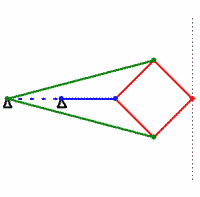
\includegraphics[scale=0.5]{15.png}

To understand the operation of the device, note it on several points:

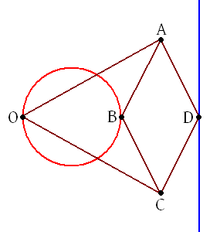
\includegraphics[scale=0.5]{16.png}

Point $B$ performs a rotation in a circle (in red), resulting in a point $D$ must move in a straight line (blue). Our task - to prove a point $D$ - The essence of the point of inversion $B$ relative to the center $O$ with a certain radius $r$.

Formalize the conditions of the problem: what is the point $O$ rigidly secured segments $OA$ and $OC$ the same, and also coincides Four segments $AB$, $BC$, $CD$, $DA$. Point $B$ moves along a circle passing through the point $O$.

For the \textbf{proof} we first note that the point $O$, $B$ and $D$ lie on a straight line (this follows from triangles). We denote $P$ point of intersection of the segments $AC$ and $BD$. We introduce the notation

$OB = x, ~ ~ ~ BP = y, ~ ~ ~ AP = h.$

We need to show that the quantity $OB \cdot OD = {\rm const}$ :

$OB \cdot OD = x (x +2 y) = x ^ 2 + 2xy.$

By the Pythagorean theorem, we obtain

$OA ^ 2 = (x + y) ^ 2 + h ^ 2,$
$AD ^ 2 = y ^ 2 + h ^ 2.$

We take the difference of these two values:

$OA ^ 2 - AD ^ 2 = x ^ 2 + 2xy = OB \cdot OD.$

Thus, we have proved that $OB \cdot OD = {\rm const}$, Which means that $D$ - Inversion point $B$.

\section{ Common tangent of two circles }
Given two circles. You want to find all of their common tangent, i.e. all such lines that relate to both circles simultaneously.

The algorithm described above will also work when one (or both) of the circle degenerates to a point. Thus, this algorithm can be used for finding the tangent to a circle passing through a given point.

\subsection{ Number of common tangents }

Just note that we do not consider \textbf{the degenerate} cases: when the circle are the same (in this case, they have infinitely many common tangents), or one circle is inside the other (in this case, they have no common tangent, or, if the circles concerned, there is one common tangent).

In most cases, the two circles have \textbf{four} common tangents.

If the circles are \textbf{concerned,} they will have three obshih tangent, but it can be understood as a degenerate case: as if the two tangents coincide.

Moreover, the algorithm described below will work in the case where one or both have zero radius of the circle: in this case will be, respectively, two or one common tangent.

In summary, we have, except for the cases described in the beginning, we will always look for \textbf{four tangents.} In degenerate cases, some of them will be the same, but nevertheless, these cases will also fit into the overall picture.

\subsection{ Algorithm }

For simplicity of the algorithm, we may assume without loss of generality, that the center of the first circle has coordinates $(0, 0)$. (If it is not, then it can achieve a simple shift of the whole picture, and after finding the solutions - Get direct shift back again.)

We denote $r_1$ and $r_2$ the radii of the first and second circles, and a $v$ - Coordinates of the center of the second circle (point $v$ different from the origin, as we do not consider the case where the circle are the same, or one circle is inside the other).

To solve the problem we come to it purely \textbf{algebraically.} We need to find all the lines of the form $ax + by + c = 0$ Which lie at a distance $r_1$ from the origin, and at a distance $r_2$ from the point of $v$. In addition, we impose the condition normalized direct sum of the squares of the coefficients $a$ and $b$ must be equal to one (this is necessary, otherwise the same line will match an infinite number of representations of the form $ax + by + c = 0$ ). Total obtain a system of equations in the unknown $a, b, c$ :

$\begin{cases}
a^{2}+b^{2}=1\\
|a\cdot0+b\cdot0+c|=r_{1}\\
|a\cdot v_{x}+b\cdot v_{y}+c|=r_{2}
\end{cases}$

To get rid of the modules, we note that there are only four ways to open the modules in the system. All of these methods can be considered a general case, if we understand how the disclosure of the module is that the coefficient on the right side may be multiplied by $-1$.

In other words, we come to such a system:

$\begin{cases}
a^{2}+b^{2}=1\\
c=\pm r_{1}\\
a\cdot v_{x}+b\cdot v_{y}+c=\pm r_{2}
\end{cases}$

Introducing the notation $d_1 = \pm r_1$ and $d_2 = \pm r_2$ We come to the fact that four times to solve the system:

$\begin{cases}
a^{2}+b^{2}=1\\
c=d_{1}\\
a\cdot v_{x}+b\cdot v_{y}+c=d_{2}
\end{cases}$

The solution of this system is reduced to solving a quadratic equation. We omit all the tedious calculations, and immediately give a ready answer:

$\begin{cases}
a=\frac{(d_{2}-d_{1})v_{x}\pm v_{y}\sqrt{v_{x}^{2}+v_{y}^{2}-(d_{2}-d_{1})^{2}}}{v_{x}^{2}+v_{y}^{2}}\\
b=\frac{(d_{2}-d_{1})v_{y}\mp v_{x}\sqrt{v_{x}^{2}+v_{y}^{2}-(d_{2}-d_{1})^{2}}}{v_{x}^{2}+v_{y}^{2}}\\
c=d_{1}
\end{cases}$

Total, we've got $8$ solutions instead $4$. But it is easy to understand, in what place there are extra solutions: in fact, in the latter system is sufficient to take only one solution (eg, the first). In fact, the geometric meaning of what we take $\pm r_1$ and $\pm r_2$, Is clear: we actually sort out which side of each of the circles will be straight. Therefore, two methods arise in the solution of the latter system, redundant: just select one of the two solutions (only, of course, in all four cases, select one and the same family of solutions).

The last thing that we have not yet considered - \textbf{this} is a \textbf{direct shift} when the first round was not initially at the origin. But here is simple: the linearity of the equation directly implies that the coefficient $c$ must subtract the value $a \cdot x_0 + b \cdot y_0$ (Where $x_0$ and $y_0$ - The coordinates of the original center of the first circle).

\subsection{ Implementation }

We first describe the necessary data structures and other auxiliary definitions:

\begin{verbatim}
struct pt {
    double x, y ;
 
    pt operator -(pt p){
        pt res = { x - p. x, y - p. y } ;
        return res ;
    }
} ;
 
struct circle : pt {
    double r ;
} ;
 
struct line {
    double a, b, c ;
} ;
 
const double EPS = 1E-9 ;
 
double sqr(double a){
    return a * a ;
} 
\end{verbatim}
Then the decision itself can be written in this way (where the main function to call - the second, and the first function - Auxiliary):

\begin{verbatim}
void tangents(pt c, double r1, double r2, vector < line > & ans){
    double r = r2 - r1 ;
    double z = sqr(c. x)+ sqr(c. y);
    double d = z - sqr(r);
    if(d < - EPS) return ;
    d = sqrt(abs(d)) ;
    line l ;
    l. a =(c. x * r + c. y * d)/ z ;
    l. b =(c. y * r - c. x * d)/ z ;
    l. c = r1 ;
    ans. push_back(l);
}
 
vector < line > tangents(circle a, circle b){
    vector < line > ans ;
    for(int i = - 1 ; i <= 1 ; i + = 2 )
        for(int j = - 1 ; j <= 1 ; j + = 2 )
            tangents(b - a, a. r * i, b. r * j, ans);
    for(size_t i = 0 ; i < ans. size() ; ++ i )
        ans[i].c - = ans[i].a * a. x + ans[i].b * a. y ;
    return ans ;
} 
\end{verbatim}
\section{ Pairs of intersecting segments (line sweep) }
Dana $n$ segments on the plane. Need to check whether the overlap with each other at least two of them. (If the answer is yes - then output the pair of intersecting segments, among quite a few answers to choose any of them.)

The naive algorithm for - sort of $O (n ^ 2)$ all pairs of intervals to check for each pair intersect or not. This article describes an algorithm with running time $O (n \log n)$, Which is based on the principle of \textbf{scanning (sweeps out) line} (in English: "sweep line").

\subsection{ Algorithm }

Draw a vertical line mentally $x = - \infty$ and begin to move this line to the right. In the course of its movement, this line will be meeting with the segments, and at any time, each segment will overlap with our direct at one point (we still assume that there is no vertical lines).

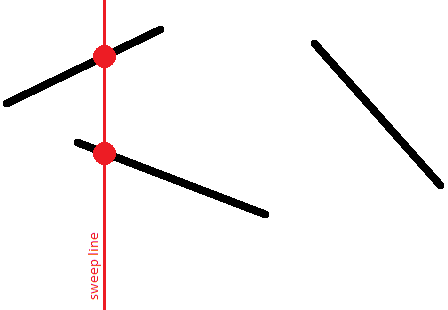
\includegraphics[scale=0.5]{17.png}

Thus, for each segment at some point it will be a point on the scanning line, then the movement will move the line and this point, and, finally, at some point in the segment will disappear from the line.

We are interested in \textbf{the relative order of the segments} vertically. Specifically, we will keep a list of segments that intersect the scanning line at a time, where the segments will be sorted by their $y$ -Coordinate on the scanning line.

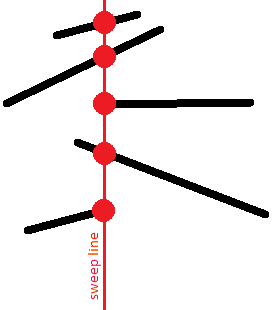
\includegraphics[scale=0.5]{18.png}

This procedure is interesting in that overlapping segments will have the same $y$ -Coordinate at least at one point in time:

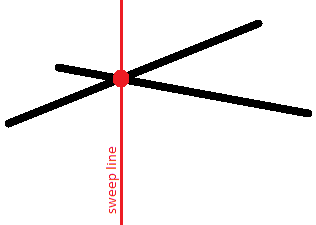
\includegraphics[scale=0.5]{19.png}

Formulate the key statements:

To search for a pair of intersecting enough to consider for each fixed position scanning direct \textbf{only the adjacent segments.}
It suffices to consider the scanning line is not valid in all possible positions $(- \infty \ldots + \infty)$ But \textbf{only in those positions when new segments or fade old.} In other words, it is sufficient to only by provisions equal abscissas-end segments.
When a new segment, simply \textbf{insert} it in the right place in the list obtained for the previous scanning line. Check on the intersection you \textbf{just add the segment with its immediate neighbors in the list of top and bottom.}
With the disappearance of the segment, simply \textbf{remove} it from the current list. After this you should \textbf{check the intersection with the upper and lower neighbors} in the list.
Other changes in the order of the segments in the list, other than those described, does not exist. Other checks on the intersection is not necessary.
To understand the truth of these assertions are the following observations:

Two non-overlapping segments never change their \textbf{relative order.}
In fact, if one piece was originally higher than the other, and then became lower, between these two moments was the intersection of these two segments.

Have matching $y$ Coordinates of two non-overlapping segments also can not.
From this it follows that at the time the interval, we can find a position in the queue for this segment, and this segment is more in line shift is not necessary: ​​its \textbf{order relative to other segments in the queue will not change.}
Two intersecting segments at their point of intersection will be \textbf{neighbors to} each other in turn.
Therefore, to find the pairs of intersecting segments is sufficient to check only to cross all those pairs of line segments, which sometime during the motion of scanning straight at least once \textbf{were neighbors of each other.}
It is easy to see that it is enough just to check the added segment with its upper and lower neighbors, as well as removing the segment - its upper and lower neighbors (which, after removal will be neighbors to each other.)

It should be noted that for a fixed position scanning the line, we \textbf{first} have to make \textbf{the addition} of all the segments appear here, and only \textbf{then} - to \textbf{remove} all the segments are endangered.
Thus, we do not miss the intersection of the segments at the top: i.e. such cases when the two segments have a common vertex.

Note that the \textbf{vertical segments} in fact does not affect the correctness of the algorithm.
These segments are distinguished by the fact that they appear and disappear at the same time. However, due to the previous remark, we know that the first all segments will be added to the queue, and only then will be removed. Consequently, if a vertical line segment intersects with any other open at this time interval (including vertical), it will be detected.

In what place queued vertical segments? After a vertical line does not have one specific $y$ Coordinates, extending for a period of at $y$ -Coordinate. But it is easy to understand that, as a $y$ Coordinates can take any coordinate of this segment.

Thus, the whole algorithm will make no more $2n$ tests intersection of a pair of segments, and will make $O (n)$ operations with a queue of segments (for $O (1)$ operations in the appearance and disappearance of each segment).

The final \textbf{asymptotic} algorithm is thus $O (n \log n)$.

\subsection{ Implementation }

We present the full implementation of the algorithm:

\begin{verbatim}
const double EPS = 1E-9 ;
 
struct pt {
    double x, y ;
} ;
 
struct seg {
    pt p, q ;
    int id ;
 
    double get_y(double x)const {
        if(abs(p. x - q. x)< EPS) return p. y ;
        return p. y +(q. y - p. y)*(x - p. x)/(q. x - p. x);
    }
} ;
 
 
inline bool intersect1d(double l1, double r1, double l2, double r2){
    if(l1 > r1) swap(l1, r1);
    if(l2 > r2) swap(l2, r2);
    return max(l1, l2)<= min(r1, r2)+ EPS ;
}
 
inline int vec(const pt & a, const pt & b, const pt & c){
    double s =(b. x - a. x)*(c. y - a. y)-(b. y - a. y)*(c. x - a. x);
    return abs(s)< EPS ? 0 : s > 0 ? + 1 : - 1 ;
}
 
bool intersect(const seg & a, const seg & b){
    return intersect1d(a. p. x, a. q. x, b. p. x, b. q. x )
        && intersect1d(a. p. y, a. q. y, b. p. y, b. q. y )
        && vec(a. p, a. q, b. p)* vec(a. p, a. q, b. q)<= 0
        && vec(b. p, b. q, a. p)* vec(b. p, b. q, a. q)<= 0 ;
}
 
 
bool operator <(const seg & a, const seg & b){
    double x = max(min(a. p. x, a. q. x ), min(b. p. x, b. q. x)) ;
    return a. get_y(x)< b. get_y(x)- EPS ;
}
 
 
struct event {
    double x ;
    int tp, id ;
 
    event() { }
    event(double x, int tp, int id )
        : x(x ), tp(tp ), id(id )
    { }
 
    bool operator <(const event & e)const {
        if(abs(x - e. x)> EPS) return x < e. x ;
        return tp > e. tp ;
    }
} ;
 
set < seg > s ;
vector < set < seg >::iterator > where ;
 
inline set < seg >::iterator prev(set < seg >::iterator it){
    return it == s. begin() ? s. end() : -- it ;
}
 
inline set < seg >::iterator next(set < seg >::iterator it){
    return ++ it ;
}
 
pair < int, int > solve(const vector < seg > & a){
    int n =(int)a. size() ;
    vector < event > e ;
    for(int i = 0 ; i < n ; ++ i){
        e. push_back(event(min(a[i].p. x, a[i].q. x ), + 1, i)) ;
        e. push_back(event(max(a[i].p. x, a[i].q. x ), - 1, i)) ;
    }
    sort(e. begin(), e. end());
 
    s. clear() ;
    where. resize(a. size());
    for(size_t i = 0 ; i < e. size() ; ++ i){
        int id = e[i].id ;
        if(e[i].tp == + 1){
            set < seg >::iterator
                nxt = s. lower_bound(a[id]),
                prv = prev(nxt);
            if(nxt ! = s. end() && intersect(* nxt, a[id ]))
                return make_pair(nxt - > id, id);
            if(prv ! = s. end() && intersect(* prv, a[id ]))
                return make_pair(prv - > id, id);
            where[id]= s. insert(nxt, a[id ]);
        }
        else {
            set < seg >::iterator
                nxt = next(where[id]),
                prv = prev(where[id ]);
            if(nxt ! = s. end() && prv ! = s. end() && intersect(* nxt, * prv))
                return make_pair(prv - > id, nxt - > id);
            s. erase(where[id ]);
        }
    }
 
return make_pair(- 1, - 1);
} 
\end{verbatim}
The main function here - $\rm solve()$, Which returns the number of the detected overlapping segments or $(-1, -1)$ If there is no intersection.

Check on the intersection of two segments are supplied by the $\rm intersect()$, Using an algorithm based on the oriented area of the triangle.

Of all the segments in the global variable $s$ - $\rm set <event>$. Iterators indicating the position of each segment in the queue (for easy removal of segments from the queue), are stored in the global array $\rm where$.

Also introduced two auxiliary functions $\rm prev()$ and $\rm next()$ That return an iterator to the next and previous elements (or $\rm end()$ If one does not exist).

Constant $\rm EPS$ denotes the error of comparing two real numbers (they are mainly used to check the intersection of two segments).
